\documentclass[]{report}

%----------
% packages
\usepackage{amsmath}
\usepackage{tikz}
\usepackage{tikz-network}

\usetikzlibrary{shapes,arrows,chains}
\usetikzlibrary[calc]
\tikzstyle{line} = [draw, -latex']
%----------
% newcommands
\newcommand{\bn}{\textbf{n}}

% Title Page
\title{}
\author{Jingyuan Sha}


\begin{document}
\maketitle

\begin{abstract}
\end{abstract}



\newpage
\chapter{Introduction}
%%%%%%%%%%%%%%%%%%%% intro %%%%%%%%%%%%%%%%%%%% 

%% What is surface normal
\section{Introduction}

Normal indicates the direction of a plane. In 3D coordinate systems, a normal is a vector, which perpendicular to the corresponding plane. Since only the direction property of a normal is demanded, the length is meaningless, thus the normal can be represented as an unit vector. In this case, each axis in range $ [-1,1] $. Therefore, for a polygon, the direction of each plane can be represented by its normal. 

%% why surface normal is important

Surface normal has many practical applications, such as augmented reality and robotics. In these applications, normal is an important basic property of object surface. Some rendering tasks such as surface reconstruction, image registration, shading, etc, they all required surface normal as one of the inputs. 

%% Surface normal from point cloud
Objects are usually captured by cameras, which provided as a single view scene with RGB colors. Some camera can also record the depth map at the same time. The depth can be converted to 3D vertices from image space. Therefore, the object in 3D space is usually represented as a point cloud. In this case, normals can not be calculated precisely since the planes of each point is unknown.



%%%%%%%%%%%%%%%%%%% talk about the reason of this thesis %%%%%%%%%%%%%%%%%%

%% standard method for normal inference is insufficient, input is sparse, not robust enough
Standard methods compute normals from point cloud using neighboring information in image space or use Shape from Shading. However, the point clouds data provided by Kinect or similar RGB-D, LiDAR sensors are only semi-dense. As shown in Figure \ref{fig:depth_map_with_noise}. If map these normals to polygon mesh, that is not good at all. 

%% add noise image
\begin{figure}[!h]
	\centering
	\begin{tikzpicture}
		\node[inner sep=0pt] (depthmap) at (0,0)
		{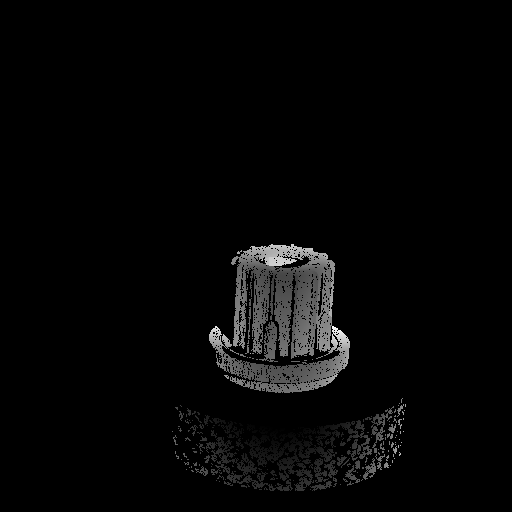
\includegraphics[width=.5\textwidth]{./pic/00028.depth0.png}};
	\end{tikzpicture}
	\caption{A depth map captured via infrared sensors. The missing pixels distributed almost all of the image.}
	\label{fig:depth_map_with_noise}
\end{figure}

Standard methods derives normal from each point and its neighborhoods' positions. It dependents on chosen neighbor size. There are two main drawbacks. First, if neighbor size is too small, it has larger noise sensitive, if it is too large, the output will too smooth and not crispy. Second, it is not robust with noise.  Errors may occur in regions with inter-reflections, where we have errors in the 3D measurement. On the other side, it is also weak with missing pixel handling, which is a common issue in depth maps.

%% add noise image
\begin{figure}[!h]
	\centering
	\begin{tikzpicture}	
		\node[inner sep=0pt] (normal) at (8,0)
		{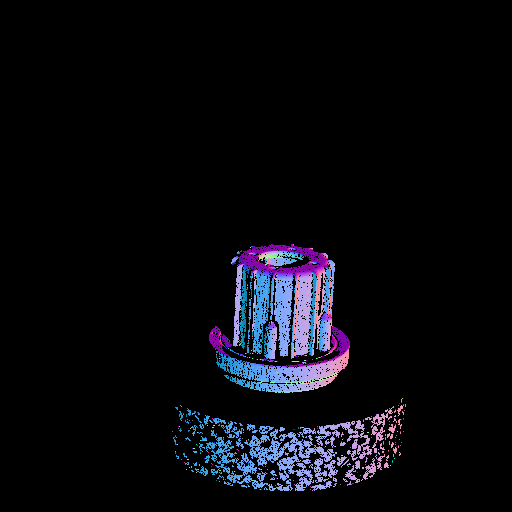
\includegraphics[width=.5\textwidth]{./pic/00028.normal0.png}};
	\end{tikzpicture}
	\caption{Semi-dense Normal Map calculated from depth map using standard method}
	\label{fig:standard_normal_inference}
\end{figure}

%% there exists space for improvment 
Although the depth image is incomplete, the depth sensor usually able to capture grayscale texture image, which are typically fully dense due to their passive nature. Furthermore, if the texture image is already illuminated by strong directional light of a video projector, whose position is known, then there should exist theoretical relations between light direction, normal direction, and grayscale image . Thus the normal can be inferenced better using the given image information and depth map. 

%%%%%%%%%%%%%%%%%%% talk about the chanllege of this task %%%%%%%%%%%%%%%%%%
Both depth and grayscale image are initially relevant to the machine learning algorithms. Based grayscale image and corresponding semi-dense depth map, a CNN model can be designed to inference the normal map, which gives more density and robust comparing to standard algorithm. However, the missing pixels in depth map can be distributed around the whole image, some of the image regions leave complete empty holes. This situation imposes further processing for the missing regions and some other challenges on the machine learning methods. 
In this thesis, we found a solution for the problems mentioned above.

%% CNN based methods
The deep convolutional neural network is typically used for image classification, which achieved great success in last several years. \cite{yolov3}, \cite{efficientDet}. 
%% talk about the reason we need new type of network architecture
These kinds of network architecture takes a single image as input which usually employed for classification problems. The image is usually convoluted with convolutional layer and downsampling with pooling layers. The outputs of the network consists of a single value to represent the ID of corresponding class \cite{efficientDet}, or with set of values to represent the position of bounding boxes.\cite{yolov3}.


However, in many other vision tasks, the output is demanded as an image, instead of predicting one or several classes of the input, but the classes of each pixel are predicted, like image segmentation\cite{unet}. In this case, the traditional network architecture is not suitable anymore.

%% improved normal inference figure
\begin{figure}[!h]
	\centering
	\begin{tikzpicture}
		
		\node[inner sep=0pt] (image) at (0,0)
		{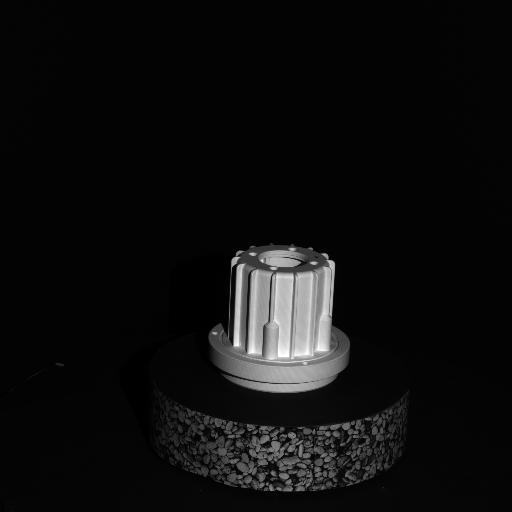
\includegraphics[width=.2\textwidth]{./pic/00028.image0.png}};
		
		\node[text width=1cm] at (2,0) {$ + $};
		
		\node[inner sep=0pt] (depthmap) at (3.3,0)
		{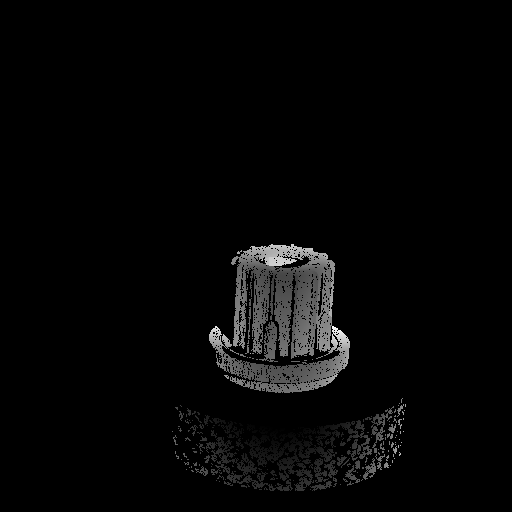
\includegraphics[width=.2\textwidth]{./pic/00028.depth0.png}};
		\node[text width=1cm] at (8,0) {$ ? $};
		
		\path [line] (5,0) -- node [text width=1cm,midway,above ] {CNN} (6,0);
		
	\end{tikzpicture}
	\caption{Left: Grayscale Image, Middle: Depth Map}
	\label{fig:improved_normal_inference}
\end{figure}


In this thesis, we proposed a novel deep learning architecture for surface normal inference. 

By applying our approach to the task of normal inference, a custom dataset is created from Unity using 3D models. The trained Normal models achieve a remarkably better prediction accuracy at a low computational cost comparing to the standard approaches for semi-dense point clouds. 























\newpage
\chapter{Related Work}


In order to estimate normals of an object surface.

In 2012, Holzer et al. \cite{Holzer.S} presented a read-time method, which is able to run algorithm in a high frame speed. They smooth the depth data in order to handle the noise of depth image. The speed is accelerated via integral image. The drawbacks are, as mentioned in the paper, the normals error go up when point depths change severely.

In 2021, Zhou et al.  \cite{zhou2021fast}





\newpage
\chapter{Approach}
\section{Dataset}
Since the images captured by Kinect usually have missing pixels, consequently, the ground truth of missing pixels are unknown. Therefore we generate synthetic 3D scene in game engine like Unity, in this case, all the information in the synthetic world can be measured, as well as normal map. Thus we captured the depth map and normal from Unity as input and ground truth. To construct the dataset, 22 3D models have been used and 1000 different scenes have been captured. Each scene has 3 images:
\begin{itemize}
	\item Depth map
	\item Grayscale image
	\item Normal Map
\end{itemize}


\begin{figure}
	\centering
	{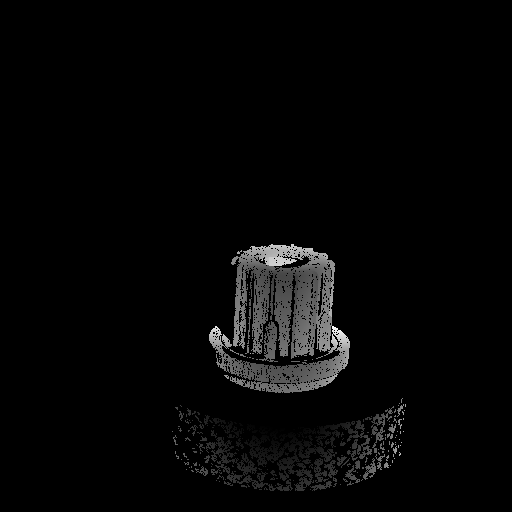
\includegraphics[width=0.4\textwidth]{./pic/00028.depth0.png}}
	\label{depth_map_kinect}
	\caption{Depth Map of an object captured by Kinect}
\end{figure}

\subsection{Noise}
The raw depth maps captured by Kinect usually have missing pixels. As shown in picture \ref{depth_map_kinect}.
Observing the depth map, the missing pixels can be divided into two groups.
\begin{itemize}
	\item random missed single pixels
	\item missed dark areas
\end{itemize}
Since the input of evaluation is incomplete Kinect depth map, thus the input of training should have the similar pattern as well. That is, adding the similar noise to synthetic depth map.
For the two kinds of depth noise, first can be simulated by adding uniformly distributed black pixels to the whole depth map, whereas the second can be dealed with a high-pass filter to filter out dark pixels and set them to 0.

%% add noise image
\begin{figure}[!h]
	\centering
	\begin{tikzpicture}
		\node[inner sep=0pt] (depthmap) at (0,0)
		{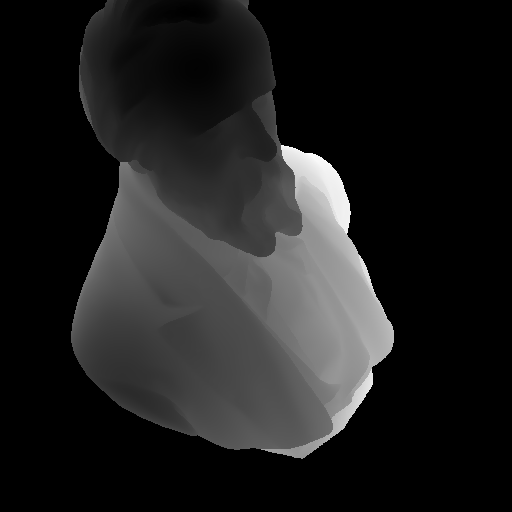
\includegraphics[width=.2\textwidth]{./pic/00440.depth0.png}};
		\draw [-stealth](2,0) -- (3,0);
		\node[inner sep=0pt] (depthmap) at (5,0)
		{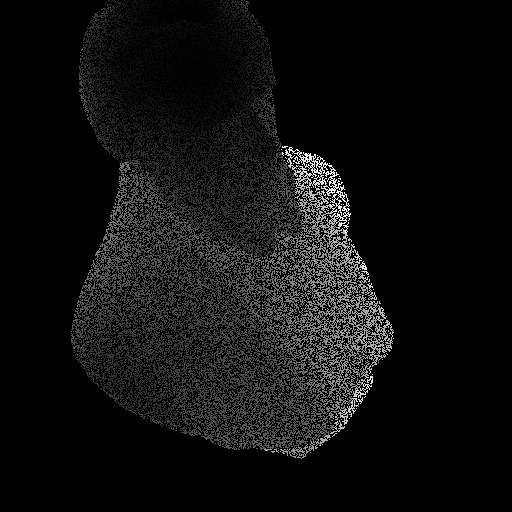
\includegraphics[width=.2\textwidth]{./pic/00440.depth0_noise.png}};
	\end{tikzpicture}
\end{figure}

Specifically, for each pixel with index $ (i,j) $ in a synthetic depth map $ D $, if its value less than a threshold $ B $, then set it to $ 0 $, i.e.
\[D(i,j) = \begin{cases}
		0 & D(i,j) \le B \\
		D(i,j) & D(i,j) > B
	\end{cases}  \]

for the rest of the pixels, the following two equal-opportunity situations will occur,
\begin{itemize}
	\item pixel value remain same
	\item pixel value set to $ 0 $
\end{itemize}





\section{Gated Convolution}

Gated Convolution layer\cite{gconv}, the output of the layer with input size $ (N, C_{in}, H, W) $ and output $ (N, C_{out}, H_{out}, W_{out}) $ can be described as:
\begin{equation}\label{gconv}
	o(N_i, C_{o_j}) = \sigma(\sum_{k=0}^{C_{in}-1}w_g(C_{o_j}, k) \star i(N_i,k) + b_g(C_{o_j})) * 
	\phi (\sum_{k=0}^{C_{in}-1}w_f(C_{o_j}, k) \star i(N_i,k) + b_f(C_{o_j}))
\end{equation}
where $ \phi $ is LeakyReLU function, $ \sigma $ is sigmoid function, thus the output values are in range $ [0,1] $, $ \star $ is the valid 2D cross-correlation operator, $ N $ is batch size, $ C $ denotes a number of channels, $ H $ is a height of input planes in pixels, and $ W $ is width in pixels, $ w(C_{o_j},k) $ denotes the weight of $ j $-th output channel corresponding $ k $-th input channel, $ i(N_i, k) $denotes the input of $ i $-th batch corresponding $ k $-th input channel, $ b(C_{o_j}) $ denotes the bias of $ j $-th output channel.




\section{Architecture}
Based on the implementation mentioned above, we propose a Gated Convolutional Neural Network to perform guided normal inference. The architecture of trained network is shown in Figure \ref{fig:cnn_archi}. There are two stages in the downsampling and one stage in upsampling. First stage takes gray scale image as input then samples downward 3 times and extracts the features using 2D convolutional layers. The second stage takes 3D vertex as input then samples downward 3 times as well but extract the features using gated convolutional layers. Then concatenate two stages together and upsampling 3 times, two standard convolutional layers have been added at the end. The output normal map has the same size as the input 3d vertex map.


\begin{figure}[!h]
	\centering

	%% https://tex.stackexchange.com/questions/12020/what-is-the-easiest-way-to-draw-a-3d-cube-with-tikz
	\begin{tikzpicture}
	%% -------------------------------------- parameters ------------------------------------------------
	\pgfmathsetmacro{\vdist}{0.7}

	\pgfmathsetmacro{\boxsizea}{3}	%% width 512
	\pgfmathsetmacro{\boxsizeb}{1.5}	%% width 256
	\pgfmathsetmacro{\boxsizec}{1}	%% width 128
	\pgfmathsetmacro{\boxsized}{0.7}	%% width 64


	\pgfmathsetmacro{\boxwidthd}{0.1}	%% width 1
	\pgfmathsetmacro{\boxwidtha}{0.3}	%% width 3
	\pgfmathsetmacro{\boxwidthb}{\boxwidtha*2}	%% width 32
	\pgfmathsetmacro{\boxwidthc}{\boxwidtha*4}		%% width 64

	\pgfmathsetmacro{\convwshift}{9}
	\pgfmathsetmacro{\preprocessingshift}{4}
	\pgfmathsetmacro{\gconvwshift}{1}

	\pgfmathsetmacro{\secrowshift}{-6}

	\pgfmathsetmacro{\convrowstart}{4}
	\pgfmathsetmacro{\secondrowstart}{4}
	\pgfmathsetmacro{\catx}{13}
	\pgfmathsetmacro{\caty}{-3.2}
	%% https://www.tug.org/pracjourn/2007-4/walden/color.pdf
	\definecolor{gconvcolor}{rgb}{0.5,0.7,0.7}
	\definecolor{convcolor}{rgb}{0.5,0.7,0.3}
	\definecolor{gconvdilatedcolor}{rgb}{0.6,0,0.3}


	%% ---------------------------------- preprocessing --------------------------------------------
	%%  img_in 1x512x512
	\pgfmathsetmacro{\disttimes}{2}
	\pgfmathsetmacro{\yschift}{\preprocessingshift}
	\node[inner sep=0pt] (depthmap) at (\vdist*\disttimes,\yschift)
	{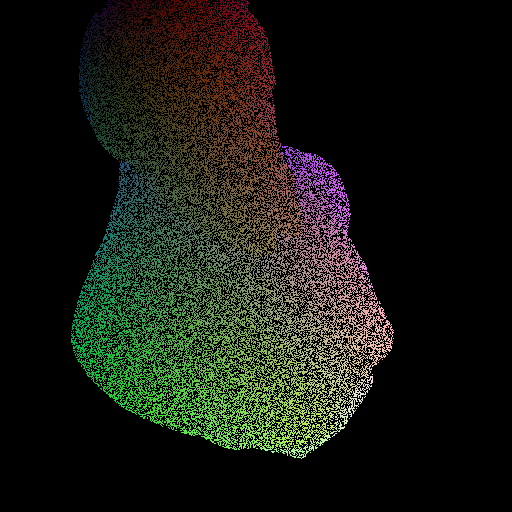
\includegraphics[width=.2\textwidth]{./pic/00440.vertex.png}};
	\node[text width=3.5cm] at (\vdist*\disttimes,\yschift-1.5) {3D Vertex};

	\draw [-stealth](\vdist*\disttimes,\yschift-1.5) -- (\vdist*\disttimes,\yschift-1.7);

	\draw [-stealth]  (\vdist*\disttimes+2,\yschift) -- (\vdist*\disttimes+1.5,\yschift);

	\pgfmathsetmacro{\disttimes}{7}
	\pgfmathsetmacro{\yschift}{\preprocessingshift}
	\node[inner sep=0pt] (depthmap) at (\vdist*\disttimes,\yschift)
	{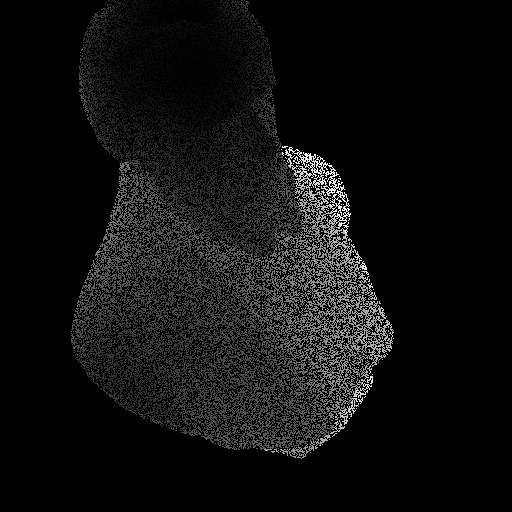
\includegraphics[width=.2\textwidth]{./pic/00440.depth0_noise.png}};
	\node[text width=3.5cm] at (\vdist*\disttimes,\yschift-1.5) {Depth Map + noise};


	\draw [-stealth] (\vdist*\disttimes+2,\yschift) -- (\vdist*\disttimes+1.5,\yschift);
	\pgfmathsetmacro{\disttimes}{12}
	\pgfmathsetmacro{\yschift}{\preprocessingshift}
	\node[inner sep=0pt] (depthmap) at (\vdist*\disttimes,\yschift)
	{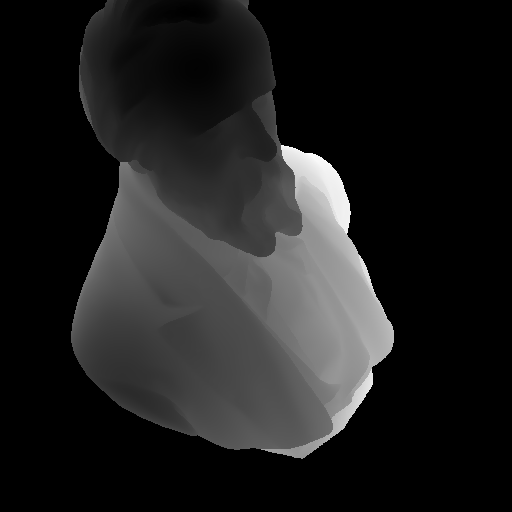
\includegraphics[width=.2\textwidth]{./pic/00440.depth0.png}};
	\node[text width=2cm] at (\vdist*\disttimes,\yschift-1.5) {Depth Map};


	%% ------------------------------------------- vertex input ----------------------------------------------
	%% 	d_in							3x512x512


	%%	dconv1: 	d_in-->x1 			32x512x512
	\pgfmathsetmacro{\disttimes}{1}	%% width 32
	\pgfmathsetmacro{\boxsize}{\boxsizea}	%% size 512
	\pgfmathsetmacro{\boxwidth}{\boxwidthb}	%% width 32
	\pgfmathsetmacro{\yschift}{\gconvwshift}
	\node[text width=1cm] at (\vdist*\disttimes+0.1,\yschift-3.5) {32};
	\draw[black, fill=gconvcolor] (\vdist*\disttimes,\yschift,0) -- ++(-\boxwidth,0,0) -- ++(0,-\boxsize,0) -- ++(\boxwidth,0,0) -- cycle;
	\draw[black, fill=gconvcolor] (\vdist*\disttimes,\yschift,0) -- ++(0,0,-\boxsize) -- ++(0,-\boxsize,0) -- ++(0,0,\boxsize) -- cycle;
	\draw[black, fill=gconvcolor] (\vdist*\disttimes,\yschift,0) -- ++(-\boxwidth,0,0) -- ++(0,0,-\boxsize) -- ++(\boxwidth,0,0) -- cycle;

	%%	dconv2:		x1-->x1				32x512x512
	\pgfmathsetmacro{\disttimes}{2}	%% width 32
	\pgfmathsetmacro{\boxsize}{\boxsizea}	%% size 512
	\pgfmathsetmacro{\boxwidth}{\boxwidthb}	%% width 32
	\pgfmathsetmacro{\yschift}{\gconvwshift}
	\draw[black, fill=gconvcolor] (\vdist*\disttimes,\yschift,0) -- ++(-\boxwidth,0,0) -- ++(0,-\boxsize,0) -- ++(\boxwidth,0,0) -- cycle;
	\draw[black, fill=gconvcolor] (\vdist*\disttimes,\yschift,0) -- ++(0,0,-\boxsize) -- ++(0,-\boxsize,0) -- ++(0,0,\boxsize) -- cycle;
	\draw[black, fill=gconvcolor] (\vdist*\disttimes,\yschift,0) -- ++(-\boxwidth,0,0) -- ++(0,0,-\boxsize) -- ++(\boxwidth,0,0) -- cycle;

	%%	dconv3:		x1-->x1				32x512x512
	\pgfmathsetmacro{\disttimes}{3}	%% width 32
	\pgfmathsetmacro{\boxsize}{\boxsizea}	%% size 512
	\pgfmathsetmacro{\boxwidth}{\boxwidthb}	%% width 32
	\pgfmathsetmacro{\yschift}{\gconvwshift}
	\draw[black, fill=gconvcolor] (\vdist*\disttimes,\yschift,0) -- ++(-\boxwidth,0,0) -- ++(0,-\boxsize,0) -- ++(\boxwidth,0,0) -- cycle;
	\draw[black, fill=gconvcolor] (\vdist*\disttimes,\yschift,0) -- ++(0,0,-\boxsize) -- ++(0,-\boxsize,0) -- ++(0,0,\boxsize) -- cycle;
	\draw[black, fill=gconvcolor] (\vdist*\disttimes,\yschift,0) -- ++(-\boxwidth,0,0) -- ++(0,0,-\boxsize) -- ++(\boxwidth,0,0) -- cycle;

	\draw (\vdist*\disttimes-0.2,\yschift-3.2) -- (\vdist*\disttimes-0.2,\yschift-4);
	\draw (\vdist*\disttimes-0.2,\yschift-4) -- (\vdist*\disttimes+5.7,\yschift-4);
	\draw [-stealth] (\vdist*\disttimes+5.7,\yschift-4) -- (\vdist*\disttimes+5.7,\yschift-5.2);
	%% downsample 1
	%%	dconv4:		x1-->x2				32x256x256
	\pgfmathsetmacro{\disttimes}{4}	%% width 32
	\pgfmathsetmacro{\boxsize}{\boxsizeb}	%% size 256
	\pgfmathsetmacro{\boxwidth}{\boxwidthb}	%% width 32
	\pgfmathsetmacro{\yschift}{\gconvwshift-0.5}	%% width 32
	\draw[black, fill=gconvcolor] (\vdist*\disttimes,\yschift,0) -- ++(-\boxwidth,0,0) -- ++(0,-\boxsize,0) -- ++(\boxwidth,0,0) -- cycle;
	\draw[black, fill=gconvcolor] (\vdist*\disttimes,\yschift,0) -- ++(0,0,-\boxsize) -- ++(0,-\boxsize,0) -- ++(0,0,\boxsize) -- cycle;
	\draw[black, fill=gconvcolor] (\vdist*\disttimes,\yschift,0) -- ++(-\boxwidth,0,0) -- ++(0,0,-\boxsize) -- ++(\boxwidth,0,0) -- cycle;
	%%	dconv2:		x2-->x2				32x256x256
	\pgfmathsetmacro{\disttimes}{5}	%% width 32
	\pgfmathsetmacro{\boxsize}{\boxsizeb}	%% size 256
	\pgfmathsetmacro{\boxwidth}{\boxwidthb}	%% width 32
	\pgfmathsetmacro{\yschift}{\gconvwshift-0.5}	%% width 32
	\draw[black, fill=gconvcolor] (\vdist*\disttimes,\yschift,0) -- ++(-\boxwidth,0,0) -- ++(0,-\boxsize,0) -- ++(\boxwidth,0,0) -- cycle;
	\draw[black, fill=gconvcolor] (\vdist*\disttimes,\yschift,0) -- ++(0,0,-\boxsize) -- ++(0,-\boxsize,0) -- ++(0,0,\boxsize) -- cycle;
	\draw[black, fill=gconvcolor] (\vdist*\disttimes,\yschift,0) -- ++(-\boxwidth,0,0) -- ++(0,0,-\boxsize) -- ++(\boxwidth,0,0) -- cycle;
	%%	dconv3:		x2-->x2				32x256x256
	\pgfmathsetmacro{\disttimes}{6}	%% width 32
	\pgfmathsetmacro{\boxsize}{\boxsizeb}	%% size 256
	\pgfmathsetmacro{\boxwidth}{\boxwidthb}	%% width 32
	\pgfmathsetmacro{\yschift}{\gconvwshift-0.5}	%% width 32
	\draw[black, fill=gconvcolor] (\vdist*\disttimes,\yschift,0) -- ++(-\boxwidth,0,0) -- ++(0,-\boxsize,0) -- ++(\boxwidth,0,0) -- cycle;
	\draw[black, fill=gconvcolor] (\vdist*\disttimes,\yschift,0) -- ++(0,0,-\boxsize) -- ++(0,-\boxsize,0) -- ++(0,0,\boxsize) -- cycle;
	\draw[black, fill=gconvcolor] (\vdist*\disttimes,\yschift,0) -- ++(-\boxwidth,0,0) -- ++(0,0,-\boxsize) -- ++(\boxwidth,0,0) -- cycle;

	\draw (\vdist*\disttimes-0.2,\yschift-1.6) -- (\vdist*\disttimes-0.2,\yschift-2.7);
	\draw (\vdist*\disttimes-0.2,\yschift-2.7) -- (\vdist*\disttimes+4.6,\yschift-2.7);
	\draw [-stealth] (\vdist*\disttimes+4.6,\yschift-2.7) -- (\vdist*\disttimes+4.6,\yschift-5.8);
	%% downsample 2
	%%	dconv4:		x2-->x3				32x128x128
	\pgfmathsetmacro{\disttimes}{7}	%% width 32
	\pgfmathsetmacro{\boxsize}{\boxsizec}	%% size 128
	\pgfmathsetmacro{\boxwidth}{\boxwidthb}	%% width 32
	\pgfmathsetmacro{\yschift}{\gconvwshift-0.8}	%% width 32
	\draw[black, fill=gconvcolor] (\vdist*\disttimes,\yschift,0) -- ++(-\boxwidth,0,0) -- ++(0,-\boxsize,0) -- ++(\boxwidth,0,0) -- cycle;
	\draw[black, fill=gconvcolor] (\vdist*\disttimes,\yschift,0) -- ++(0,0,-\boxsize) -- ++(0,-\boxsize,0) -- ++(0,0,\boxsize) -- cycle;
	\draw[black, fill=gconvcolor] (\vdist*\disttimes,\yschift,0) -- ++(-\boxwidth,0,0) -- ++(0,0,-\boxsize) -- ++(\boxwidth,0,0) -- cycle;
	%%	dconv2:		x3-->x3				32x128x128
	\pgfmathsetmacro{\disttimes}{8}	%% width 32
	\pgfmathsetmacro{\boxsize}{\boxsizec}	%% size 128
	\pgfmathsetmacro{\boxwidth}{\boxwidthb}	%% width 32
	\pgfmathsetmacro{\yschift}{\gconvwshift-0.8}	%% width 32
	\draw[black, fill=gconvcolor] (\vdist*\disttimes,\yschift,0) -- ++(-\boxwidth,0,0) -- ++(0,-\boxsize,0) -- ++(\boxwidth,0,0) -- cycle;
	\draw[black, fill=gconvcolor] (\vdist*\disttimes,\yschift,0) -- ++(0,0,-\boxsize) -- ++(0,-\boxsize,0) -- ++(0,0,\boxsize) -- cycle;
	\draw[black, fill=gconvcolor] (\vdist*\disttimes,\yschift,0) -- ++(-\boxwidth,0,0) -- ++(0,0,-\boxsize) -- ++(\boxwidth,0,0) -- cycle;
	%%	dconv3:		x3-->x3				32x128x128
	\pgfmathsetmacro{\disttimes}{9}	%% width 32
	\pgfmathsetmacro{\boxsize}{\boxsizec}	%% size 128
	\pgfmathsetmacro{\boxwidth}{\boxwidthb}	%% width 32
	\pgfmathsetmacro{\yschift}{\gconvwshift-0.8}	%% width 32
	\draw[black, fill=gconvcolor] (\vdist*\disttimes,\yschift,0) -- ++(-\boxwidth,0,0) -- ++(0,-\boxsize,0) -- ++(\boxwidth,0,0) -- cycle;
	\draw[black, fill=gconvcolor] (\vdist*\disttimes,\yschift,0) -- ++(0,0,-\boxsize) -- ++(0,-\boxsize,0) -- ++(0,0,\boxsize) -- cycle;
	\draw[black, fill=gconvcolor] (\vdist*\disttimes,\yschift,0) -- ++(-\boxwidth,0,0) -- ++(0,0,-\boxsize) -- ++(\boxwidth,0,0) -- cycle;
	%% downsample 3
	%%	dconv4:		x3-->x4				32x64x64
	\pgfmathsetmacro{\disttimes}{10}
	\pgfmathsetmacro{\boxsize}{\boxsized}	%% size 64
	\pgfmathsetmacro{\boxwidth}{\boxwidthb}	%% width 32
	\pgfmathsetmacro{\yschift}{\gconvwshift-1}
	\draw[black, fill=gconvcolor] (\vdist*\disttimes,\yschift,0) -- ++(-\boxwidth,0,0) -- ++(0,-\boxsize,0) -- ++(\boxwidth,0,0) -- cycle;
	\draw[black, fill=gconvcolor] (\vdist*\disttimes,\yschift,0) -- ++(0,0,-\boxsize) -- ++(0,-\boxsize,0) -- ++(0,0,\boxsize) -- cycle;
	\draw[black, fill=gconvcolor] (\vdist*\disttimes,\yschift,0) -- ++(-\boxwidth,0,0) -- ++(0,0,-\boxsize) -- ++(\boxwidth,0,0) -- cycle;
	%%	dconv2:		x4-->x4				32x64x64
	\pgfmathsetmacro{\disttimes}{11}
	\pgfmathsetmacro{\boxsize}{\boxsized}	%% size 64
	\pgfmathsetmacro{\boxwidth}{\boxwidthb}	%% width 32
	\pgfmathsetmacro{\yschift}{\gconvwshift-1}	%% width 32
	\draw[black, fill=gconvcolor] (\vdist*\disttimes,\yschift,0) -- ++(-\boxwidth,0,0) -- ++(0,-\boxsize,0) -- ++(\boxwidth,0,0) -- cycle;
	\draw[black, fill=gconvcolor] (\vdist*\disttimes,\yschift,0) -- ++(0,0,-\boxsize) -- ++(0,-\boxsize,0) -- ++(0,0,\boxsize) -- cycle;
	\draw[black, fill=gconvcolor] (\vdist*\disttimes,\yschift,0) -- ++(-\boxwidth,0,0) -- ++(0,0,-\boxsize) -- ++(\boxwidth,0,0) -- cycle;
	%%	dconv3:		x4-->x4				32x64x64
	\pgfmathsetmacro{\disttimes}{12}
	\pgfmathsetmacro{\boxsize}{\boxsized}	%% size 64
	\pgfmathsetmacro{\boxwidth}{\boxwidthb}	%% width 32
	\pgfmathsetmacro{\yschift}{\gconvwshift-1}	%% width 32
	\draw[black, fill=gconvcolor] (\vdist*\disttimes,\yschift,0) -- ++(-\boxwidth,0,0) -- ++(0,-\boxsize,0) -- ++(\boxwidth,0,0) -- cycle;
	\draw[black, fill=gconvcolor] (\vdist*\disttimes,\yschift,0) -- ++(0,0,-\boxsize) -- ++(0,-\boxsize,0) -- ++(0,0,\boxsize) -- cycle;
	\draw[black, fill=gconvcolor] (\vdist*\disttimes,\yschift,0) -- ++(-\boxwidth,0,0) -- ++(0,0,-\boxsize) -- ++(\boxwidth,0,0) -- cycle;

	%% dilated
	%%	dilated1:	x4-->x4				32x64x64
	\pgfmathsetmacro{\disttimes}{13}
	\pgfmathsetmacro{\boxsize}{\boxsized}	%% size 64
	\pgfmathsetmacro{\boxwidth}{\boxwidthb}	%% width 32
	\pgfmathsetmacro{\yschift}{\gconvwshift-1}	%% width 32
	\draw[black, fill=gconvdilatedcolor] (\vdist*\disttimes,\yschift,0) -- ++(-\boxwidth,0,0) -- ++(0,-\boxsize,0) -- ++(\boxwidth,0,0) -- cycle;
	\draw[black, fill=gconvdilatedcolor] (\vdist*\disttimes,\yschift,0) -- ++(0,0,-\boxsize) -- ++(0,-\boxsize,0) -- ++(0,0,\boxsize) -- cycle;
	\draw[black, fill=gconvdilatedcolor] (\vdist*\disttimes,\yschift,0) -- ++(-\boxwidth,0,0) -- ++(0,0,-\boxsize) -- ++(\boxwidth,0,0) -- cycle;
	%%	dilated2:	x4-->x4				32x64x64
	\pgfmathsetmacro{\disttimes}{14}
	\pgfmathsetmacro{\boxsize}{\boxsized}	%% size 64
	\pgfmathsetmacro{\boxwidth}{\boxwidthb}	%% width 32
	\pgfmathsetmacro{\yschift}{\gconvwshift-1}	%% width 32
	\draw[black, fill=gconvdilatedcolor] (\vdist*\disttimes,\yschift,0) -- ++(-\boxwidth,0,0) -- ++(0,-\boxsize,0) -- ++(\boxwidth,0,0) -- cycle;
	\draw[black, fill=gconvdilatedcolor] (\vdist*\disttimes,\yschift,0) -- ++(0,0,-\boxsize) -- ++(0,-\boxsize,0) -- ++(0,0,\boxsize) -- cycle;
	\draw[black, fill=gconvdilatedcolor] (\vdist*\disttimes,\yschift,0) -- ++(-\boxwidth,0,0) -- ++(0,0,-\boxsize) -- ++(\boxwidth,0,0) -- cycle;
	%%	dilated3:	x4-->x4				32x64x64
	\pgfmathsetmacro{\disttimes}{15}
	\pgfmathsetmacro{\boxsize}{\boxsized}	%% size 64
	\pgfmathsetmacro{\boxwidth}{\boxwidthb}	%% width 32
	\pgfmathsetmacro{\yschift}{\gconvwshift-1}	%% width 32
	\draw[black, fill=gconvdilatedcolor] (\vdist*\disttimes,\yschift,0) -- ++(-\boxwidth,0,0) -- ++(0,-\boxsize,0) -- ++(\boxwidth,0,0) -- cycle;
	\draw[black, fill=gconvdilatedcolor] (\vdist*\disttimes,\yschift,0) -- ++(0,0,-\boxsize) -- ++(0,-\boxsize,0) -- ++(0,0,\boxsize) -- cycle;
	\draw[black, fill=gconvdilatedcolor] (\vdist*\disttimes,\yschift,0) -- ++(-\boxwidth,0,0) -- ++(0,0,-\boxsize) -- ++(\boxwidth,0,0) -- cycle;
	%%	dilated4:	x4-->x4				32x64x64
	\pgfmathsetmacro{\disttimes}{16}
	\pgfmathsetmacro{\boxsize}{\boxsized}	%% size 64
	\pgfmathsetmacro{\boxwidth}{\boxwidthb}	%% width 32
	\pgfmathsetmacro{\yschift}{\gconvwshift-1}	%% width 32
	\draw[black, fill=gconvdilatedcolor] (\vdist*\disttimes,\yschift,0) -- ++(-\boxwidth,0,0) -- ++(0,-\boxsize,0) -- ++(\boxwidth,0,0) -- cycle;
	\draw[black, fill=gconvdilatedcolor] (\vdist*\disttimes,\yschift,0) -- ++(0,0,-\boxsize) -- ++(0,-\boxsize,0) -- ++(0,0,\boxsize) -- cycle;
	\draw[black, fill=gconvdilatedcolor] (\vdist*\disttimes,\yschift,0) -- ++(-\boxwidth,0,0) -- ++(0,0,-\boxsize) -- ++(\boxwidth,0,0) -- cycle;
	%%	dconv2:		x4-->x4				32x64x64
	\pgfmathsetmacro{\disttimes}{17}
	\pgfmathsetmacro{\boxsize}{\boxsized}	%% size 64
	\pgfmathsetmacro{\boxwidth}{\boxwidthb}	%% width 32
	\pgfmathsetmacro{\yschift}{\gconvwshift-1}	%% width 32
	\draw[black, fill=gconvcolor] (\vdist*\disttimes,\yschift,0) -- ++(-\boxwidth,0,0) -- ++(0,-\boxsize,0) -- ++(\boxwidth,0,0) -- cycle;
	\draw[black, fill=gconvcolor] (\vdist*\disttimes,\yschift,0) -- ++(0,0,-\boxsize) -- ++(0,-\boxsize,0) -- ++(0,0,\boxsize) -- cycle;
	\draw[black, fill=gconvcolor] (\vdist*\disttimes,\yschift,0) -- ++(-\boxwidth,0,0) -- ++(0,0,-\boxsize) -- ++(\boxwidth,0,0) -- cycle;
	%%	dconv3:		x4-->x4				32x64x64
	\pgfmathsetmacro{\disttimes}{18}
	\pgfmathsetmacro{\boxsize}{\boxsized}	%% size 64
	\pgfmathsetmacro{\boxwidth}{\boxwidthb}	%% width 32
	\pgfmathsetmacro{\yschift}{\gconvwshift-1}	%% width 32
	\draw[black, fill=gconvcolor] (\vdist*\disttimes,\yschift,0) -- ++(-\boxwidth,0,0) -- ++(0,-\boxsize,0) -- ++(\boxwidth,0,0) -- cycle;
	\draw[black, fill=gconvcolor] (\vdist*\disttimes,\yschift,0) -- ++(0,0,-\boxsize) -- ++(0,-\boxsize,0) -- ++(0,0,\boxsize) -- cycle;
	\draw[black, fill=gconvcolor] (\vdist*\disttimes,\yschift,0) -- ++(-\boxwidth,0,0) -- ++(0,0,-\boxsize) -- ++(\boxwidth,0,0) -- cycle;

	\draw (\vdist*\disttimes+0.25,\yschift-0.25) -- (\catx,\yschift-0.25);
	\draw [-stealth](\catx,\yschift-0.25) -- (\catx,\caty);




	%% ------------------------------ img feature ----------------------------------------------------------------

	\pgfmathsetmacro{\disttimes}{0}
	\pgfmathsetmacro{\yschift}{\convwshift-1}
	\node[inner sep=0pt] (depthmap) at (\vdist*\disttimes,\yschift)
	{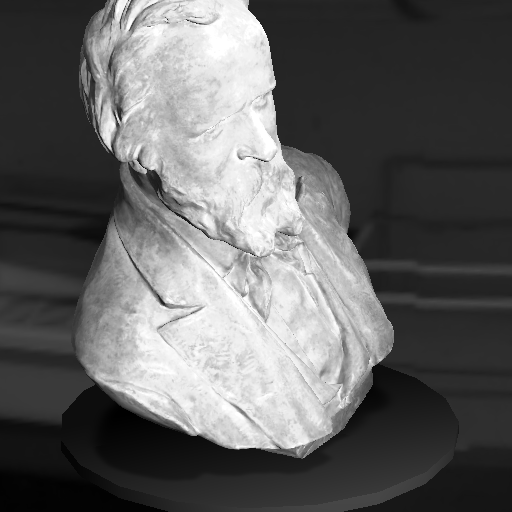
\includegraphics[width=.2\textwidth]{./pic/00440.image0.png}};
	\node[text width=3cm] at (\vdist*\disttimes,\yschift-1.5) {Gray Scale Image};
	\draw [-stealth](\vdist*\disttimes+1.5,\yschift) -- (\vdist*\disttimes+2.5,\yschift);

	%%	img_conv1:	img_in-->x_img_1 	32x512x512
	\pgfmathsetmacro{\disttimes}{\convrowstart + 1}
	\pgfmathsetmacro{\boxsize}{\boxsizea}	%% size 512
	\pgfmathsetmacro{\boxwidth}{\boxwidthb}	%% width 32
	\pgfmathsetmacro{\yschift}{\convwshift}
	\draw[black, fill=convcolor] (\vdist*\disttimes,\yschift,0) -- ++(-\boxwidth,0,0) -- ++(0,-\boxsize,0) -- ++(\boxwidth,0,0) -- cycle;
	\draw[black, fill=convcolor] (\vdist*\disttimes,\yschift,0) -- ++(0,0,-\boxsize) -- ++(0,-\boxsize,0) -- ++(0,0,\boxsize) -- cycle;
	\draw[black, fill=convcolor] (\vdist*\disttimes,\yschift,0) -- ++(-\boxwidth,0,0) -- ++(0,0,-\boxsize) -- ++(\boxwidth,0,0) -- cycle;
	%%	img_conv2:	x_img_1-->x_img_1	32x512x512
	\pgfmathsetmacro{\disttimes}{\convrowstart+2}	%% width 32
	\pgfmathsetmacro{\boxsize}{\boxsizea}	%% size 512
	\pgfmathsetmacro{\boxwidth}{\boxwidthb}	%% width 32
	\pgfmathsetmacro{\yschift}{\convwshift}
	\draw[black, fill=convcolor] (\vdist*\disttimes,\yschift,0) -- ++(-\boxwidth,0,0) -- ++(0,-\boxsize,0) -- ++(\boxwidth,0,0) -- cycle;
	\draw[black, fill=convcolor] (\vdist*\disttimes,\yschift,0) -- ++(0,0,-\boxsize) -- ++(0,-\boxsize,0) -- ++(0,0,\boxsize) -- cycle;
	\draw[black, fill=convcolor] (\vdist*\disttimes,\yschift,0) -- ++(-\boxwidth,0,0) -- ++(0,0,-\boxsize) -- ++(\boxwidth,0,0) -- cycle;
	%%	img_conv3:	x_img_1-->x_img_1	32x512x512
	\pgfmathsetmacro{\disttimes}{\convrowstart+3}	%% width 32
	\pgfmathsetmacro{\boxsize}{\boxsizea}	%% size 256
	\pgfmathsetmacro{\boxwidth}{\boxwidthb}	%% width 32
	\pgfmathsetmacro{\yschift}{\convwshift}
	\draw[black, fill=convcolor] (\vdist*\disttimes,\yschift,0) -- ++(-\boxwidth,0,0) -- ++(0,-\boxsize,0) -- ++(\boxwidth,0,0) -- cycle;
	\draw[black, fill=convcolor] (\vdist*\disttimes,\yschift,0) -- ++(0,0,-\boxsize) -- ++(0,-\boxsize,0) -- ++(0,0,\boxsize) -- cycle;
	\draw[black, fill=convcolor] (\vdist*\disttimes,\yschift,0) -- ++(-\boxwidth,0,0) -- ++(0,0,-\boxsize) -- ++(\boxwidth,0,0) -- cycle;

	%% downsample 1
	%%	img_conv4:	x_img_1-->x_img_2 	32x256x256
	\pgfmathsetmacro{\disttimes}{\convrowstart+4}
	\pgfmathsetmacro{\boxsize}{\boxsizeb}	%% size 256
	\pgfmathsetmacro{\boxwidth}{\boxwidthb}	%% width 32
	\pgfmathsetmacro{\yschift}{\convwshift-0.5}
	\draw[black, fill=convcolor] (\vdist*\disttimes,\yschift,0) -- ++(-\boxwidth,0,0) -- ++(0,-\boxsize,0) -- ++(\boxwidth,0,0) -- cycle;
	\draw[black, fill=convcolor] (\vdist*\disttimes,\yschift,0) -- ++(0,0,-\boxsize) -- ++(0,-\boxsize,0) -- ++(0,0,\boxsize) -- cycle;
	\draw[black, fill=convcolor] (\vdist*\disttimes,\yschift,0) -- ++(-\boxwidth,0,0) -- ++(0,0,-\boxsize) -- ++(\boxwidth,0,0) -- cycle;
	%%	img_conv2:	x_img_2-->x_img_2	32x256x256
	\pgfmathsetmacro{\disttimes}{\convrowstart+5}
	\pgfmathsetmacro{\boxsize}{\boxsizeb}	%% size 256
	\pgfmathsetmacro{\boxwidth}{\boxwidthb}	%% width 32
	\pgfmathsetmacro{\yschift}{\convwshift-.5}
	\draw[black, fill=convcolor] (\vdist*\disttimes,\yschift,0) -- ++(-\boxwidth,0,0) -- ++(0,-\boxsize,0) -- ++(\boxwidth,0,0) -- cycle;
	\draw[black, fill=convcolor] (\vdist*\disttimes,\yschift,0) -- ++(0,0,-\boxsize) -- ++(0,-\boxsize,0) -- ++(0,0,\boxsize) -- cycle;
	\draw[black, fill=convcolor] (\vdist*\disttimes,\yschift,0) -- ++(-\boxwidth,0,0) -- ++(0,0,-\boxsize) -- ++(\boxwidth,0,0) -- cycle;
	%%	img_conv3:	x_img_2-->x_img_2	32x256x256
	\pgfmathsetmacro{\disttimes}{\convrowstart+6}
	\pgfmathsetmacro{\boxsize}{\boxsizeb}	%% size 256
	\pgfmathsetmacro{\boxwidth}{\boxwidthb}	%% width 32
	\pgfmathsetmacro{\yschift}{\convwshift-0.5}
	\draw[black, fill=convcolor] (\vdist*\disttimes,\yschift,0) -- ++(-\boxwidth,0,0) -- ++(0,-\boxsize,0) -- ++(\boxwidth,0,0) -- cycle;
	\draw[black, fill=convcolor] (\vdist*\disttimes,\yschift,0) -- ++(0,0,-\boxsize) -- ++(0,-\boxsize,0) -- ++(0,0,\boxsize) -- cycle;
	\draw[black, fill=convcolor] (\vdist*\disttimes,\yschift,0) -- ++(-\boxwidth,0,0) -- ++(0,0,-\boxsize) -- ++(\boxwidth,0,0) -- cycle;

	%% downsample 2
	%%	img_conv4:	x_img_2-->x_img_3 	32x128x128
	\pgfmathsetmacro{\disttimes}{\convrowstart+7}
	\pgfmathsetmacro{\boxsize}{\boxsizec}	%% size 128
	\pgfmathsetmacro{\boxwidth}{\boxwidthb}	%% width 32
	\pgfmathsetmacro{\yschift}{\convwshift-1}
	\draw[black, fill=convcolor] (\vdist*\disttimes,\yschift,0) -- ++(-\boxwidth,0,0) -- ++(0,-\boxsize,0) -- ++(\boxwidth,0,0) -- cycle;
	\draw[black, fill=convcolor] (\vdist*\disttimes,\yschift,0) -- ++(0,0,-\boxsize) -- ++(0,-\boxsize,0) -- ++(0,0,\boxsize) -- cycle;
	\draw[black, fill=convcolor] (\vdist*\disttimes,\yschift,0) -- ++(-\boxwidth,0,0) -- ++(0,0,-\boxsize) -- ++(\boxwidth,0,0) -- cycle;
	%%	img_conv2:	x_img_3-->x_img_3	32x128x128
	\pgfmathsetmacro{\disttimes}{\convrowstart+8}
	\pgfmathsetmacro{\boxsize}{\boxsizec}	%% size 128
	\pgfmathsetmacro{\boxwidth}{\boxwidthb}	%% width 32
	\pgfmathsetmacro{\yschift}{\convwshift-1}
	\draw[black, fill=convcolor] (\vdist*\disttimes,\yschift,0) -- ++(-\boxwidth,0,0) -- ++(0,-\boxsize,0) -- ++(\boxwidth,0,0) -- cycle;
	\draw[black, fill=convcolor] (\vdist*\disttimes,\yschift,0) -- ++(0,0,-\boxsize) -- ++(0,-\boxsize,0) -- ++(0,0,\boxsize) -- cycle;
	\draw[black, fill=convcolor] (\vdist*\disttimes,\yschift,0) -- ++(-\boxwidth,0,0) -- ++(0,0,-\boxsize) -- ++(\boxwidth,0,0) -- cycle;
	%%	img_conv3:	x_img_3-->x_img_3	32x128x128
	\pgfmathsetmacro{\disttimes}{\convrowstart+9}
	\pgfmathsetmacro{\boxsize}{\boxsizec}	%% size 128
	\pgfmathsetmacro{\boxwidth}{\boxwidthb}	%% width 32
	\pgfmathsetmacro{\yschift}{\convwshift-1}
	\draw[black, fill=convcolor] (\vdist*\disttimes,\yschift,0) -- ++(-\boxwidth,0,0) -- ++(0,-\boxsize,0) -- ++(\boxwidth,0,0) -- cycle;
	\draw[black, fill=convcolor] (\vdist*\disttimes,\yschift,0) -- ++(0,0,-\boxsize) -- ++(0,-\boxsize,0) -- ++(0,0,\boxsize) -- cycle;
	\draw[black, fill=convcolor] (\vdist*\disttimes,\yschift,0) -- ++(-\boxwidth,0,0) -- ++(0,0,-\boxsize) -- ++(\boxwidth,0,0) -- cycle;

	%% downsample 3
	%%	img_conv4:	x_img_3-->x_img_4 	32x64x64
	\pgfmathsetmacro{\disttimes}{\convrowstart+10}
	\pgfmathsetmacro{\boxsize}{\boxsized}	%% size 64
	\pgfmathsetmacro{\boxwidth}{\boxwidthb}	%% width 32
	\pgfmathsetmacro{\yschift}{\convwshift-1.25}
	\draw[black, fill=convcolor] (\vdist*\disttimes,\yschift,0) -- ++(-\boxwidth,0,0) -- ++(0,-\boxsize,0) -- ++(\boxwidth,0,0) -- cycle;
	\draw[black, fill=convcolor] (\vdist*\disttimes,\yschift,0) -- ++(0,0,-\boxsize) -- ++(0,-\boxsize,0) -- ++(0,0,\boxsize) -- cycle;
	\draw[black, fill=convcolor] (\vdist*\disttimes,\yschift,0) -- ++(-\boxwidth,0,0) -- ++(0,0,-\boxsize) -- ++(\boxwidth,0,0) -- cycle;
	%%	img_conv2:	x_img_4-->x_img_4	32x64x64
	\pgfmathsetmacro{\disttimes}{\convrowstart+11}
	\pgfmathsetmacro{\boxsize}{\boxsized}	%% size 64
	\pgfmathsetmacro{\boxwidth}{\boxwidthb}	%% width 32
	\pgfmathsetmacro{\yschift}{\convwshift-1.25}
	\draw[black, fill=convcolor] (\vdist*\disttimes,\yschift,0) -- ++(-\boxwidth,0,0) -- ++(0,-\boxsize,0) -- ++(\boxwidth,0,0) -- cycle;
	\draw[black, fill=convcolor] (\vdist*\disttimes,\yschift,0) -- ++(0,0,-\boxsize) -- ++(0,-\boxsize,0) -- ++(0,0,\boxsize) -- cycle;
	\draw[black, fill=convcolor] (\vdist*\disttimes,\yschift,0) -- ++(-\boxwidth,0,0) -- ++(0,0,-\boxsize) -- ++(\boxwidth,0,0) -- cycle;
	%%	img_conv3:	x_img_4-->x_img_4	32x64x64
	\pgfmathsetmacro{\disttimes}{\convrowstart+12}
	\pgfmathsetmacro{\boxsize}{\boxsized}	%% size 64
	\pgfmathsetmacro{\boxwidth}{\boxwidthb}	%% width 32
	\pgfmathsetmacro{\yschift}{\convwshift-1.25}
	\draw[black, fill=convcolor] (\vdist*\disttimes,\yschift,0) -- ++(-\boxwidth,0,0) -- ++(0,-\boxsize,0) -- ++(\boxwidth,0,0) -- cycle;
	\draw[black, fill=convcolor] (\vdist*\disttimes,\yschift,0) -- ++(0,0,-\boxsize) -- ++(0,-\boxsize,0) -- ++(0,0,\boxsize) -- cycle;
	\draw[black, fill=convcolor] (\vdist*\disttimes,\yschift,0) -- ++(-\boxwidth,0,0) -- ++(0,0,-\boxsize) -- ++(\boxwidth,0,0) -- cycle;


	\draw (\vdist*\disttimes+0.25,\yschift-0.25) -- (\catx+\boxwidth,\yschift-0.25);
	\draw [-stealth](\catx+\boxwidth,\yschift-0.25) -- (\catx+\boxwidth,\caty);

	%% ----------------------------------------- merge ------------------------------------------------------------------------------
	%%			x4,x_img_4-->x4			64x64x64

	\pgfmathsetmacro{\disttimes}{20}
	%% x4
	\pgfmathsetmacro{\boxsize}{\boxsized}	%% size 64
	\pgfmathsetmacro{\boxwidth}{\boxwidthb}	%% width 32
	\pgfmathsetmacro{\yschift}{\caty}
	\draw[black, fill=gconvcolor] (\catx,\yschift,0) -- ++(-\boxwidth,0,0) -- ++(0,-\boxsize,0) -- ++(\boxwidth,0,0) -- cycle;
	\draw[black, fill=gconvcolor] (\catx,\yschift,0) -- ++(0,0,-\boxsize) -- ++(0,-\boxsize,0) -- ++(0,0,\boxsize) -- cycle;
	\draw[black, fill=gconvcolor] (\catx,\yschift,0) -- ++(-\boxwidth,0,0) -- ++(0,0,-\boxsize) -- ++(\boxwidth,0,0) -- cycle;
	%% x_img_4
	\pgfmathsetmacro{\boxsize}{\boxsized}	%% size 64
	\pgfmathsetmacro{\boxwidth}{\boxwidthb}	%% width 32
	\pgfmathsetmacro{\yschift}{\caty}	%% width 32
	\draw[black, fill=convcolor] (\catx+\boxwidth,\yschift,0) -- ++(-\boxwidth,0,0) -- ++(0,-\boxsize,0) -- ++(\boxwidth,0,0) -- cycle;
	\draw[black, fill=convcolor] (\catx+\boxwidth,\yschift,0) -- ++(0,0,-\boxsize) -- ++(0,-\boxsize,0) -- ++(0,0,\boxsize) -- cycle;
	\draw[black, fill=convcolor] (\catx+\boxwidth,\yschift,0) -- ++(-\boxwidth,0,0) -- ++(0,0,-\boxsize) -- ++(\boxwidth,0,0) -- cycle;


	\node[text width=1cm] at (\catx,\caty-1) {concatenate};


	%% --------------------------------------------- output normal map --------------------------------------------------------------------
	\pgfmathsetmacro{\disttimes}{2.3}
	\pgfmathsetmacro{\yschift}{\secrowshift-0.5}
	\node[inner sep=0pt] (depthmap) at (\vdist*\disttimes,\yschift)
	{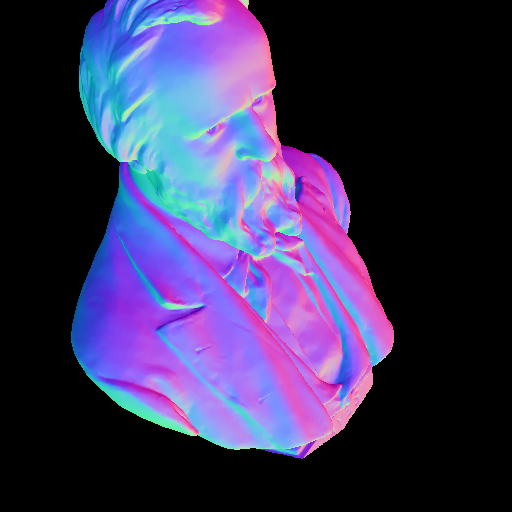
\includegraphics[width=.2\textwidth]{./pic/00440.normal0.png}};
	\node[text width=2cm] at (\vdist*\disttimes,\yschift-1.5) {Normal Map};

	\draw [-stealth] (\vdist*\disttimes+2.5,\yschift) -- (\vdist*\disttimes+2,\yschift);


	%% ------------------------------------- output ----------------------------------------------------------------------------------------
	%% conv2		xout-->xout			3x512x512
	\pgfmathsetmacro{\disttimes}{\secondrowstart + 3}
	\pgfmathsetmacro{\boxsize}{\boxsizea}	%% size 512
	\pgfmathsetmacro{\boxwidth}{\boxwidtha}	%% width 3
	\pgfmathsetmacro{\yschift}{\secrowshift+0.5}	%% width 32
	\draw[black, fill=convcolor] (\vdist*\disttimes,\yschift,0) -- ++(-\boxwidth,0,0) -- ++(0,-\boxsize,0) -- ++(\boxwidth,0,0) -- cycle;
	\draw[black, fill=convcolor] (\vdist*\disttimes,\yschift,0) -- ++(0,0,-\boxsize) -- ++(0,-\boxsize,0) -- ++(0,0,\boxsize) -- cycle;
	\draw[black, fill=convcolor] (\vdist*\disttimes,\yschift,0) -- ++(-\boxwidth,0,0) -- ++(0,0,-\boxsize) -- ++(\boxwidth,0,0) -- cycle;


	%% conv1		x1-->xout			3x512x512
	\pgfmathsetmacro{\disttimes}{\secondrowstart + 4}
	\pgfmathsetmacro{\boxsize}{\boxsizea}	%% size 512
	\pgfmathsetmacro{\boxwidth}{\boxwidtha}	%% width 3
	\pgfmathsetmacro{\yschift}{\secrowshift+0.5}	%% width 32
	\node[text width=1cm] at (\vdist*\disttimes+0.4,\yschift-2.2) {3};
	\draw[black, fill=convcolor] (\vdist*\disttimes,\yschift,0) -- ++(-\boxwidth,0,0) -- ++(0,-\boxsize,0) -- ++(\boxwidth,0,0) -- cycle;
	\draw[black, fill=convcolor] (\vdist*\disttimes,\yschift,0) -- ++(0,0,-\boxsize) -- ++(0,-\boxsize,0) -- ++(0,0,\boxsize) -- cycle;
	\draw[black, fill=convcolor] (\vdist*\disttimes,\yschift,0) -- ++(-\boxwidth,0,0) -- ++(0,0,-\boxsize) -- ++(\boxwidth,0,0) -- cycle;


	%% ----------------------------------------------------------------------------------------------------------------------
	%% uconv3		x1,x1_us-->x1		32x512x512
	\pgfmathsetmacro{\disttimes}{\secondrowstart + 5}
	\pgfmathsetmacro{\boxsize}{\boxsizea}	%% size 512
	\pgfmathsetmacro{\boxwidth}{\boxwidthb}	%% width 32
	\pgfmathsetmacro{\yschift}{\secrowshift+0.5}	%% width 32
	\draw[black, fill=gconvcolor] (\vdist*\disttimes,\yschift,0) -- ++(-\boxwidth,0,0) -- ++(0,-\boxsize,0) -- ++(\boxwidth,0,0) -- cycle;
	\draw[black, fill=gconvcolor] (\vdist*\disttimes,\yschift,0) -- ++(0,0,-\boxsize) -- ++(0,-\boxsize,0) -- ++(0,0,\boxsize) -- cycle;
	\draw[black, fill=gconvcolor] (\vdist*\disttimes,\yschift,0) -- ++(-\boxwidth,0,0) -- ++(0,0,-\boxsize) -- ++(\boxwidth,0,0) -- cycle;

	%% upsample 3
	%% interpolate	x2-->x1_us			32x512x512
	\pgfmathsetmacro{\disttimes}{\secondrowstart + 6}
	\pgfmathsetmacro{\boxsize}{\boxsizea}	%% size 512
	\pgfmathsetmacro{\boxwidth}{\boxwidthb}	%% width 32
	\pgfmathsetmacro{\yschift}{\secrowshift+0.5}	%% width 32
	\draw[black, fill=gconvcolor] (\vdist*\disttimes,\yschift,0) -- ++(-\boxwidth,0,0) -- ++(0,-\boxsize,0) -- ++(\boxwidth,0,0) -- cycle;
	\draw[black, fill=gconvcolor] (\vdist*\disttimes,\yschift,0) -- ++(0,0,-\boxsize) -- ++(0,-\boxsize,0) -- ++(0,0,\boxsize) -- cycle;
	\draw[black, fill=gconvcolor] (\vdist*\disttimes,\yschift,0) -- ++(-\boxwidth,0,0) -- ++(0,0,-\boxsize) -- ++(\boxwidth,0,0) -- cycle;
	\pgfmathsetmacro{\boxsize}{\boxsizea}	%% size 512
	\pgfmathsetmacro{\boxwidth}{\boxwidthb}	%% width 32
	\pgfmathsetmacro{\yschift}{\secrowshift+0.5}	%% width 32
	\draw[black, fill=gconvcolor] (\vdist*\disttimes+\boxwidth,\yschift,0) -- ++(-\boxwidth,0,0) -- ++(0,-\boxsize,0) -- ++(\boxwidth,0,0) -- cycle;
	\draw[black, fill=gconvcolor] (\vdist*\disttimes+\boxwidth,\yschift,0) -- ++(0,0,-\boxsize) -- ++(0,-\boxsize,0) -- ++(0,0,\boxsize) -- cycle;
	\draw[black, fill=gconvcolor] (\vdist*\disttimes+\boxwidth,\yschift,0) -- ++(-\boxwidth,0,0) -- ++(0,0,-\boxsize) -- ++(\boxwidth,0,0) -- cycle;

	%% uconv2		x2,x2_us-->x2		32x256x256
	\pgfmathsetmacro{\disttimes}{\secondrowstart + 8}
	\pgfmathsetmacro{\boxsize}{\boxsizeb}	%% size 256
	\pgfmathsetmacro{\boxwidth}{\boxwidthb}	%% width 32
	\pgfmathsetmacro{\yschift}{\secrowshift}	%% width 32
	\draw[black, fill=gconvcolor] (\vdist*\disttimes,\yschift,0) -- ++(-\boxwidth,0,0) -- ++(0,-\boxsize,0) -- ++(\boxwidth,0,0) -- cycle;
	\draw[black, fill=gconvcolor] (\vdist*\disttimes,\yschift,0) -- ++(0,0,-\boxsize) -- ++(0,-\boxsize,0) -- ++(0,0,\boxsize) -- cycle;
	\draw[black, fill=gconvcolor] (\vdist*\disttimes,\yschift,0) -- ++(-\boxwidth,0,0) -- ++(0,0,-\boxsize) -- ++(\boxwidth,0,0) -- cycle;

	\pgfmathsetmacro{\boxsize}{\boxsizeb}	%% size 256
	\pgfmathsetmacro{\boxwidth}{\boxwidthb}	%% width 32
	\pgfmathsetmacro{\yschift}{\secrowshift}	%% width 32
	\draw[black, fill=gconvcolor] (\vdist*\disttimes+\boxwidth,\yschift,0) -- ++(-\boxwidth,0,0) -- ++(0,-\boxsize,0) -- ++(\boxwidth,0,0) -- cycle;
	\draw[black, fill=gconvcolor] (\vdist*\disttimes+\boxwidth,\yschift,0) -- ++(0,0,-\boxsize) -- ++(0,-\boxsize,0) -- ++(0,0,\boxsize) -- cycle;
	\draw[black, fill=gconvcolor] (\vdist*\disttimes+\boxwidth,\yschift,0) -- ++(-\boxwidth,0,0) -- ++(0,0,-\boxsize) -- ++(\boxwidth,0,0) -- cycle;

	%% upsample 2
	%% interpolate	x3-->x2_us			32x256x256
	\pgfmathsetmacro{\disttimes}{\secondrowstart + 10}
	\pgfmathsetmacro{\boxsize}{\boxsizeb}	%% size 256
	\pgfmathsetmacro{\boxwidth}{\boxwidthb}	%% width 32
	\pgfmathsetmacro{\yschift}{\secrowshift}	%% width 32
	\draw[black, fill=gconvcolor] (\vdist*\disttimes,\yschift,0) -- ++(-\boxwidth,0,0) -- ++(0,-\boxsize,0) -- ++(\boxwidth,0,0) -- cycle;
	\draw[black, fill=gconvcolor] (\vdist*\disttimes,\yschift,0) -- ++(0,0,-\boxsize) -- ++(0,-\boxsize,0) -- ++(0,0,\boxsize) -- cycle;
	\draw[black, fill=gconvcolor] (\vdist*\disttimes,\yschift,0) -- ++(-\boxwidth,0,0) -- ++(0,0,-\boxsize) -- ++(\boxwidth,0,0) -- cycle;

	%% uconv1		x3_us-->x3			32x128x128
	\pgfmathsetmacro{\disttimes}{\secondrowstart + 12}
	\pgfmathsetmacro{\boxsize}{\boxsizec}	%% size 128
	\pgfmathsetmacro{\boxwidth}{\boxwidthb}	%% width 32
	\pgfmathsetmacro{\yschift}{\secrowshift}	%% width 32
	\node[text width=1cm] at (\vdist*\disttimes+0.2,\yschift-1.5) {32};
	\draw[black, fill=gconvcolor] (\vdist*\disttimes,\yschift,0) -- ++(-\boxwidth,0,0) -- ++(0,-\boxsize,0) -- ++(\boxwidth,0,0) -- cycle;
	\draw[black, fill=gconvcolor] (\vdist*\disttimes,\yschift,0) -- ++(0,0,-\boxsize) -- ++(0,-\boxsize,0) -- ++(0,0,\boxsize) -- cycle;
	\draw[black, fill=gconvcolor] (\vdist*\disttimes,\yschift,0) -- ++(-\boxwidth,0,0) -- ++(0,0,-\boxsize) -- ++(\boxwidth,0,0) -- cycle;

	%% upsample 1
	%% interpolate	x4-->x3_us			64x128x128
	\pgfmathsetmacro{\disttimes}{\secondrowstart +14}
	\pgfmathsetmacro{\boxsize}{\boxsizec}	%% size 128
	\pgfmathsetmacro{\boxwidth}{\boxwidthc}	%% width 64
	\pgfmathsetmacro{\yschift}{\secrowshift}	%% width 32
	\node[text width=1cm] at (\vdist*\disttimes,\yschift-1.5) {64};
	\draw[black, fill=gconvcolor] (\vdist*\disttimes,\yschift,0) -- ++(-\boxwidth,0,0) -- ++(0,-\boxsize,0) -- ++(\boxwidth,0,0) -- cycle;
	\draw[black, fill=gconvcolor] (\vdist*\disttimes,\yschift,0) -- ++(0,0,-\boxsize) -- ++(0,-\boxsize,0) -- ++(0,0,\boxsize) -- cycle;
	\draw[black, fill=gconvcolor] (\vdist*\disttimes,\yschift,0) -- ++(-\boxwidth,0,0) -- ++(0,0,-\boxsize) -- ++(\boxwidth,0,0) -- cycle;

	\draw (\catx+0.3,\caty-1.3) -- (\catx+0.3,\secrowshift);
	\draw [-stealth] (\catx+0.3,\secrowshift) -- (\secondrowstart +9,\secrowshift);
\end{tikzpicture}

	\caption{CNN Architecture}
	\label{fig:cnn_archi}
\end{figure}










				




\newpage
\chapter{Experiments}
The model is trained with PyTorch 1.10.2, CUDA 10.2.89, GPU with single NVIDIA GEFORCE GTX 1080Ti.


%% nnn24 exp
\section{Neighbor Input}


%% nnnn exp
\section{Normal Neural Network}
The first neural network that worked well for normal prediction in this master thesis is introduced in this section. It is simply named Normal Neural Network, or NNN. The input is 512x512x3 3D vertex matrix and output is 512x512x3 normal map. The architecture is based on UNet \cite{unet} with 3 times downsampling and 3 times upsampling. Gated convolution layer is used as a substitution for standard convolution layer in order to handle the sparse input. The channel size is 32 through the whole network unless the last one.  
For the training detail, this model is trained on the whole dataset with 500 items, with learning rate 0.001, penalty 1.4. The model architecture is shown in Figure \ref{fig:nnnn_archi}


\begin{figure}[!h]
	\centering
	
	%% https://tex.stackexchange.com/questions/12020/what-is-the-easiest-way-to-draw-a-3d-cube-with-tikz
	\begin{tikzpicture}
		%% -------------------------------------- parameters ------------------------------------------------
		\pgfmathsetmacro{\vdist}{0.4}
		
		\pgfmathsetmacro{\boxsizea}{3}	%% width 512
		\pgfmathsetmacro{\boxsizeb}{1.5}	%% width 256
		\pgfmathsetmacro{\boxsizec}{1}	%% width 128
		\pgfmathsetmacro{\boxsized}{0.7}	%% width 64
		
		
		\pgfmathsetmacro{\boxwidthd}{0.1}	%% width 1
		\pgfmathsetmacro{\boxwidtha}{0.2}	%% width 3
		\pgfmathsetmacro{\boxwidthb}{\boxwidtha*1.3}	%% width 32
		\pgfmathsetmacro{\boxwidthc}{\boxwidtha*3}		%% width 64
		
		\pgfmathsetmacro{\convwshift}{9}
		\pgfmathsetmacro{\preprocessingshift}{4}
		\pgfmathsetmacro{\labelshift}{1.5}
		\pgfmathsetmacro{\gconvwshift}{0}
		
		\pgfmathsetmacro{\secrowshift}{-6}
		
		\pgfmathsetmacro{\convrowstart}{4}
		\pgfmathsetmacro{\secondrowstart}{4}

		%% https://www.tug.org/pracjourn/2007-4/walden/color.pdf
		\definecolor{gconvcolor}{rgb}{0.5,0.7,0.7}
		\definecolor{convcolor}{rgb}{0.5,0.7,0.3}
		\definecolor{gconvdilatedcolor}{rgb}{0.6,0,0.3}
		
		
		%% ---------------------------------- preprocessing --------------------------------------------
		%%  img_in 1x512x512
		\pgfmathsetmacro{\disttimes}{3.5}
		\pgfmathsetmacro{\yschift}{\preprocessingshift}
		\node[inner sep=0pt] (depthmap) at (\vdist*\disttimes,\yschift)
		{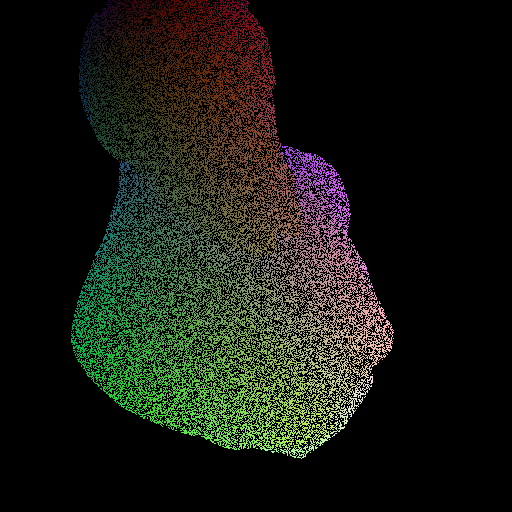
\includegraphics[width=.15\textwidth]{./pic/00440.vertex.png}};
		\node[text width=3.5cm] at (\vdist*\disttimes+1,\yschift-1.5) {3D Vertex};
		
		\draw [-stealth](1.45,\yschift-1.8) -- (1.45,\yschift-2.6);
		
		\draw [-stealth]  (\vdist*\disttimes+1.6,\yschift) -- (\vdist*\disttimes+1.1,\yschift);
		
		\pgfmathsetmacro{\disttimes}{10}
		\pgfmathsetmacro{\yschift}{\preprocessingshift}
		\node[inner sep=0pt] (depthmap) at (\vdist*\disttimes,\yschift)
		{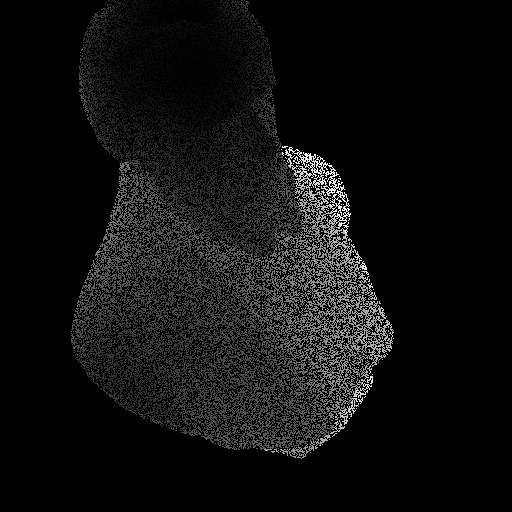
\includegraphics[width=.15\textwidth]{./pic/00440.depth0_noise.png}};
		\node[text width=3.5cm] at (\vdist*\disttimes+1,\yschift-1.5) {Add Noise};
		
		\draw [-stealth] (\vdist*\disttimes+1.6,\yschift) -- (\vdist*\disttimes+1.1,\yschift);
		
		\pgfmathsetmacro{\disttimes}{16.5}
		\pgfmathsetmacro{\yschift}{\preprocessingshift}
		\node[inner sep=0pt] (depthmap) at (\vdist*\disttimes,\yschift)
		{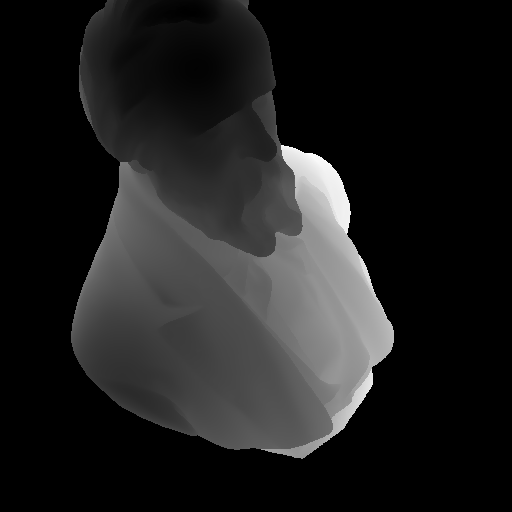
\includegraphics[width=.15\textwidth]{./pic/00440.depth0.png}};
		\node[text width=2cm] at (\vdist*\disttimes+0.2,\yschift-1.5) {Depth Map};
		
		
		%% ----------------------------------- output normal map -------------------------------------
		\pgfmathsetmacro{\disttimes}{31}
		\pgfmathsetmacro{\yschift}{\preprocessingshift}
		\node[inner sep=0pt] (depthmap) at (\vdist*\disttimes,\yschift)
		{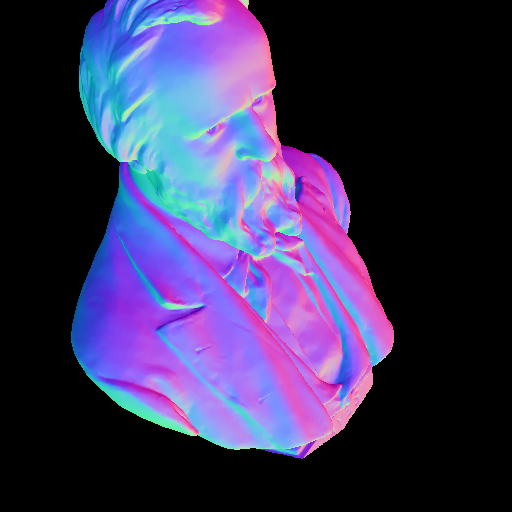
\includegraphics[width=.15\textwidth]{./pic/00440.normal0.png}};
		\node[text width=2cm] at (\vdist*\disttimes,\yschift-1.5) {Normal Map};
		
		\draw [-stealth] (\vdist*\disttimes+0.2,\yschift-2.7) -- (\vdist*\disttimes+0.2,\yschift-1.8);
		
		
		%% ------------------------------------------- vertex input ----------------------------------------------
		%% 	d_in							3x512x512
		%%	dconv1: 	d_in-->x1 			32x512x512
		\pgfmathsetmacro{\disttimes}{1}	%% width 32
		\pgfmathsetmacro{\boxsize}{\boxsizea}	%% size 512
		\pgfmathsetmacro{\boxwidth}{\boxwidthb}	%% width 32
		\pgfmathsetmacro{\yschift}{\gconvwshift}
		\node[text width=1cm] at (\vdist*\disttimes+0.1,\yschift-3.5) {32};
		\draw[black, fill=gconvcolor] (\vdist*\disttimes,\yschift,0) -- ++(-\boxwidth,0,0) -- ++(0,-\boxsize,0) -- ++(\boxwidth,0,0) -- cycle;
		\draw[black, fill=gconvcolor] (\vdist*\disttimes,\yschift,0) -- ++(0,0,-\boxsize) -- ++(0,-\boxsize,0) -- ++(0,0,\boxsize) -- cycle;
		\draw[black, fill=gconvcolor] (\vdist*\disttimes,\yschift,0) -- ++(-\boxwidth,0,0) -- ++(0,0,-\boxsize) -- ++(\boxwidth,0,0) -- cycle;
		
		%%	dconv2:		x1-->x1				32x512x512
		\pgfmathsetmacro{\disttimes}{2}	%% width 32
		\pgfmathsetmacro{\boxsize}{\boxsizea}	%% size 512
		\pgfmathsetmacro{\boxwidth}{\boxwidthb}	%% width 32
		\pgfmathsetmacro{\yschift}{\gconvwshift}
		\draw[black, fill=gconvcolor] (\vdist*\disttimes,\yschift,0) -- ++(-\boxwidth,0,0) -- ++(0,-\boxsize,0) -- ++(\boxwidth,0,0) -- cycle;
		\draw[black, fill=gconvcolor] (\vdist*\disttimes,\yschift,0) -- ++(0,0,-\boxsize) -- ++(0,-\boxsize,0) -- ++(0,0,\boxsize) -- cycle;
		\draw[black, fill=gconvcolor] (\vdist*\disttimes,\yschift,0) -- ++(-\boxwidth,0,0) -- ++(0,0,-\boxsize) -- ++(\boxwidth,0,0) -- cycle;
		
		%%	dconv3:		x1-->x1				32x512x512
		\pgfmathsetmacro{\disttimes}{3}	%% width 32
		\pgfmathsetmacro{\boxsize}{\boxsizea}	%% size 512
		\pgfmathsetmacro{\boxwidth}{\boxwidthb}	%% width 32
		\pgfmathsetmacro{\yschift}{\gconvwshift}
		\draw[black, fill=gconvcolor] (\vdist*\disttimes,\yschift,0) -- ++(-\boxwidth,0,0) -- ++(0,-\boxsize,0) -- ++(\boxwidth,0,0) -- cycle;
		\draw[black, fill=gconvcolor] (\vdist*\disttimes,\yschift,0) -- ++(0,0,-\boxsize) -- ++(0,-\boxsize,0) -- ++(0,0,\boxsize) -- cycle;
		\draw[black, fill=gconvcolor] (\vdist*\disttimes,\yschift,0) -- ++(-\boxwidth,0,0) -- ++(0,0,-\boxsize) -- ++(\boxwidth,0,0) -- cycle;
		
		\draw (\vdist*\disttimes-0.2,\yschift-3.2) -- (\vdist*\disttimes-0.2,\yschift-4);
		\draw (\vdist*\disttimes-0.2,\yschift-4) -- (\vdist*\disttimes+9,\yschift-4);
		\draw [-stealth] (\vdist*\disttimes+9,\yschift-4) -- (\vdist*\disttimes+9,\yschift-3.2);
		
		
		%% downsample 1
		%%	dconv4:		x1-->x2				32x256x256
		\pgfmathsetmacro{\disttimes}{4}	%% width 32
		\pgfmathsetmacro{\boxsize}{\boxsizeb}	%% size 256
		\pgfmathsetmacro{\boxwidth}{\boxwidthb}	%% width 32
		\pgfmathsetmacro{\yschift}{\gconvwshift-0.5}	%% width 32
		\draw[black, fill=gconvcolor] (\vdist*\disttimes,\yschift,0) -- ++(-\boxwidth,0,0) -- ++(0,-\boxsize,0) -- ++(\boxwidth,0,0) -- cycle;
		\draw[black, fill=gconvcolor] (\vdist*\disttimes,\yschift,0) -- ++(0,0,-\boxsize) -- ++(0,-\boxsize,0) -- ++(0,0,\boxsize) -- cycle;
		\draw[black, fill=gconvcolor] (\vdist*\disttimes,\yschift,0) -- ++(-\boxwidth,0,0) -- ++(0,0,-\boxsize) -- ++(\boxwidth,0,0) -- cycle;
		%%	dconv2:		x2-->x2				32x256x256
		\pgfmathsetmacro{\disttimes}{5}	%% width 32
		\pgfmathsetmacro{\boxsize}{\boxsizeb}	%% size 256
		\pgfmathsetmacro{\boxwidth}{\boxwidthb}	%% width 32
		\pgfmathsetmacro{\yschift}{\gconvwshift-0.5}	%% width 32
		\draw[black, fill=gconvcolor] (\vdist*\disttimes,\yschift,0) -- ++(-\boxwidth,0,0) -- ++(0,-\boxsize,0) -- ++(\boxwidth,0,0) -- cycle;
		\draw[black, fill=gconvcolor] (\vdist*\disttimes,\yschift,0) -- ++(0,0,-\boxsize) -- ++(0,-\boxsize,0) -- ++(0,0,\boxsize) -- cycle;
		\draw[black, fill=gconvcolor] (\vdist*\disttimes,\yschift,0) -- ++(-\boxwidth,0,0) -- ++(0,0,-\boxsize) -- ++(\boxwidth,0,0) -- cycle;
		%%	dconv3:		x2-->x2				32x256x256
		\pgfmathsetmacro{\disttimes}{6}	%% width 32
		\pgfmathsetmacro{\boxsize}{\boxsizeb}	%% size 256
		\pgfmathsetmacro{\boxwidth}{\boxwidthb}	%% width 32
		\pgfmathsetmacro{\yschift}{\gconvwshift-0.5}	%% width 32
		\draw[black, fill=gconvcolor] (\vdist*\disttimes,\yschift,0) -- ++(-\boxwidth,0,0) -- ++(0,-\boxsize,0) -- ++(\boxwidth,0,0) -- cycle;
		\draw[black, fill=gconvcolor] (\vdist*\disttimes,\yschift,0) -- ++(0,0,-\boxsize) -- ++(0,-\boxsize,0) -- ++(0,0,\boxsize) -- cycle;
		\draw[black, fill=gconvcolor] (\vdist*\disttimes,\yschift,0) -- ++(-\boxwidth,0,0) -- ++(0,0,-\boxsize) -- ++(\boxwidth,0,0) -- cycle;
		
		\draw (\vdist*\disttimes-0.1,\yschift-1.6) -- (\vdist*\disttimes-0.1,\yschift-2.7);
		\draw (\vdist*\disttimes-0.1,\yschift-2.7) -- (\vdist*\disttimes+6.5,\yschift-2.7);
		\draw [-stealth] (\vdist*\disttimes+6.5,\yschift-2.7) -- (\vdist*\disttimes+6.5,\yschift-1.7);
		
		
		%% downsample 2
		%%	dconv4:		x2-->x3				32x128x128
		\pgfmathsetmacro{\disttimes}{7}	%% width 32
		\pgfmathsetmacro{\boxsize}{\boxsizec}	%% size 128
		\pgfmathsetmacro{\boxwidth}{\boxwidthb}	%% width 32
		\pgfmathsetmacro{\yschift}{\gconvwshift-0.8}	%% width 32
		\draw[black, fill=gconvcolor] (\vdist*\disttimes,\yschift,0) -- ++(-\boxwidth,0,0) -- ++(0,-\boxsize,0) -- ++(\boxwidth,0,0) -- cycle;
		\draw[black, fill=gconvcolor] (\vdist*\disttimes,\yschift,0) -- ++(0,0,-\boxsize) -- ++(0,-\boxsize,0) -- ++(0,0,\boxsize) -- cycle;
		\draw[black, fill=gconvcolor] (\vdist*\disttimes,\yschift,0) -- ++(-\boxwidth,0,0) -- ++(0,0,-\boxsize) -- ++(\boxwidth,0,0) -- cycle;
		%%	dconv2:		x3-->x3				32x128x128
		\pgfmathsetmacro{\disttimes}{8}	%% width 32
		\pgfmathsetmacro{\boxsize}{\boxsizec}	%% size 128
		\pgfmathsetmacro{\boxwidth}{\boxwidthb}	%% width 32
		\pgfmathsetmacro{\yschift}{\gconvwshift-0.8}	%% width 32
		\draw[black, fill=gconvcolor] (\vdist*\disttimes,\yschift,0) -- ++(-\boxwidth,0,0) -- ++(0,-\boxsize,0) -- ++(\boxwidth,0,0) -- cycle;
		\draw[black, fill=gconvcolor] (\vdist*\disttimes,\yschift,0) -- ++(0,0,-\boxsize) -- ++(0,-\boxsize,0) -- ++(0,0,\boxsize) -- cycle;
		\draw[black, fill=gconvcolor] (\vdist*\disttimes,\yschift,0) -- ++(-\boxwidth,0,0) -- ++(0,0,-\boxsize) -- ++(\boxwidth,0,0) -- cycle;
		%%	dconv3:		x3-->x3				32x128x128
		\pgfmathsetmacro{\disttimes}{9}	%% width 32
		\pgfmathsetmacro{\boxsize}{\boxsizec}	%% size 128
		\pgfmathsetmacro{\boxwidth}{\boxwidthb}	%% width 32
		\pgfmathsetmacro{\yschift}{\gconvwshift-0.8}	%% width 32
		\draw[black, fill=gconvcolor] (\vdist*\disttimes,\yschift,0) -- ++(-\boxwidth,0,0) -- ++(0,-\boxsize,0) -- ++(\boxwidth,0,0) -- cycle;
		\draw[black, fill=gconvcolor] (\vdist*\disttimes,\yschift,0) -- ++(0,0,-\boxsize) -- ++(0,-\boxsize,0) -- ++(0,0,\boxsize) -- cycle;
		\draw[black, fill=gconvcolor] (\vdist*\disttimes,\yschift,0) -- ++(-\boxwidth,0,0) -- ++(0,0,-\boxsize) -- ++(\boxwidth,0,0) -- cycle;
		
		\draw (\vdist*\disttimes-0.1,\yschift-1.2) -- (\vdist*\disttimes-0.1,\yschift-1.8);
		\draw (\vdist*\disttimes-0.1,\yschift-1.8) -- (\vdist*\disttimes+4.2,\yschift-1.8);
		\draw [-stealth] (\vdist*\disttimes+4.2,\yschift-1.8) -- (\vdist*\disttimes+4.2,\yschift-1.2);
		
		
		%% downsample 3
		%%	dconv4:		x3-->x4				32x64x64
		\pgfmathsetmacro{\disttimes}{10}
		\pgfmathsetmacro{\boxsize}{\boxsized}	%% size 64
		\pgfmathsetmacro{\boxwidth}{\boxwidthb}	%% width 32
		\pgfmathsetmacro{\yschift}{\gconvwshift-1}
		\draw[black, fill=gconvcolor] (\vdist*\disttimes,\yschift,0) -- ++(-\boxwidth,0,0) -- ++(0,-\boxsize,0) -- ++(\boxwidth,0,0) -- cycle;
		\draw[black, fill=gconvcolor] (\vdist*\disttimes,\yschift,0) -- ++(0,0,-\boxsize) -- ++(0,-\boxsize,0) -- ++(0,0,\boxsize) -- cycle;
		\draw[black, fill=gconvcolor] (\vdist*\disttimes,\yschift,0) -- ++(-\boxwidth,0,0) -- ++(0,0,-\boxsize) -- ++(\boxwidth,0,0) -- cycle;
		%%	dconv2:		x4-->x4				32x64x64
		\pgfmathsetmacro{\disttimes}{11}
		\pgfmathsetmacro{\boxsize}{\boxsized}	%% size 64
		\pgfmathsetmacro{\boxwidth}{\boxwidthb}	%% width 32
		\pgfmathsetmacro{\yschift}{\gconvwshift-1}	%% width 32
		\draw[black, fill=gconvcolor] (\vdist*\disttimes,\yschift,0) -- ++(-\boxwidth,0,0) -- ++(0,-\boxsize,0) -- ++(\boxwidth,0,0) -- cycle;
		\draw[black, fill=gconvcolor] (\vdist*\disttimes,\yschift,0) -- ++(0,0,-\boxsize) -- ++(0,-\boxsize,0) -- ++(0,0,\boxsize) -- cycle;
		\draw[black, fill=gconvcolor] (\vdist*\disttimes,\yschift,0) -- ++(-\boxwidth,0,0) -- ++(0,0,-\boxsize) -- ++(\boxwidth,0,0) -- cycle;
		%%	dconv3:		x4-->x4				32x64x64
		\pgfmathsetmacro{\disttimes}{12}
		\pgfmathsetmacro{\boxsize}{\boxsized}	%% size 64
		\pgfmathsetmacro{\boxwidth}{\boxwidthb}	%% width 32
		\pgfmathsetmacro{\yschift}{\gconvwshift-1}	%% width 32
		\draw[black, fill=gconvcolor] (\vdist*\disttimes,\yschift,0) -- ++(-\boxwidth,0,0) -- ++(0,-\boxsize,0) -- ++(\boxwidth,0,0) -- cycle;
		\draw[black, fill=gconvcolor] (\vdist*\disttimes,\yschift,0) -- ++(0,0,-\boxsize) -- ++(0,-\boxsize,0) -- ++(0,0,\boxsize) -- cycle;
		\draw[black, fill=gconvcolor] (\vdist*\disttimes,\yschift,0) -- ++(-\boxwidth,0,0) -- ++(0,0,-\boxsize) -- ++(\boxwidth,0,0) -- cycle;
		
		%% dilated
		%%	dilated1:	x4-->x4				32x64x64
		\pgfmathsetmacro{\disttimes}{13}
		\pgfmathsetmacro{\boxsize}{\boxsized}	%% size 64
		\pgfmathsetmacro{\boxwidth}{\boxwidthb}	%% width 32
		\pgfmathsetmacro{\yschift}{\gconvwshift-1}	%% width 32
		\draw[black, fill=gconvdilatedcolor] (\vdist*\disttimes,\yschift,0) -- ++(-\boxwidth,0,0) -- ++(0,-\boxsize,0) -- ++(\boxwidth,0,0) -- cycle;
		\draw[black, fill=gconvdilatedcolor] (\vdist*\disttimes,\yschift,0) -- ++(0,0,-\boxsize) -- ++(0,-\boxsize,0) -- ++(0,0,\boxsize) -- cycle;
		\draw[black, fill=gconvdilatedcolor] (\vdist*\disttimes,\yschift,0) -- ++(-\boxwidth,0,0) -- ++(0,0,-\boxsize) -- ++(\boxwidth,0,0) -- cycle;
		%%	dilated2:	x4-->x4				32x64x64
		\pgfmathsetmacro{\disttimes}{14}
		\pgfmathsetmacro{\boxsize}{\boxsized}	%% size 64
		\pgfmathsetmacro{\boxwidth}{\boxwidthb}	%% width 32
		\pgfmathsetmacro{\yschift}{\gconvwshift-1}	%% width 32
		\draw[black, fill=gconvdilatedcolor] (\vdist*\disttimes,\yschift,0) -- ++(-\boxwidth,0,0) -- ++(0,-\boxsize,0) -- ++(\boxwidth,0,0) -- cycle;
		\draw[black, fill=gconvdilatedcolor] (\vdist*\disttimes,\yschift,0) -- ++(0,0,-\boxsize) -- ++(0,-\boxsize,0) -- ++(0,0,\boxsize) -- cycle;
		\draw[black, fill=gconvdilatedcolor] (\vdist*\disttimes,\yschift,0) -- ++(-\boxwidth,0,0) -- ++(0,0,-\boxsize) -- ++(\boxwidth,0,0) -- cycle;
		%%	dilated3:	x4-->x4				32x64x64
		\pgfmathsetmacro{\disttimes}{15}
		\pgfmathsetmacro{\boxsize}{\boxsized}	%% size 64
		\pgfmathsetmacro{\boxwidth}{\boxwidthb}	%% width 32
		\pgfmathsetmacro{\yschift}{\gconvwshift-1}	%% width 32
		\draw[black, fill=gconvdilatedcolor] (\vdist*\disttimes,\yschift,0) -- ++(-\boxwidth,0,0) -- ++(0,-\boxsize,0) -- ++(\boxwidth,0,0) -- cycle;
		\draw[black, fill=gconvdilatedcolor] (\vdist*\disttimes,\yschift,0) -- ++(0,0,-\boxsize) -- ++(0,-\boxsize,0) -- ++(0,0,\boxsize) -- cycle;
		\draw[black, fill=gconvdilatedcolor] (\vdist*\disttimes,\yschift,0) -- ++(-\boxwidth,0,0) -- ++(0,0,-\boxsize) -- ++(\boxwidth,0,0) -- cycle;
		%%	dilated4:	x4-->x4				32x64x64
		\pgfmathsetmacro{\disttimes}{16}
		\pgfmathsetmacro{\boxsize}{\boxsized}	%% size 64
		\pgfmathsetmacro{\boxwidth}{\boxwidthb}	%% width 32
		\pgfmathsetmacro{\yschift}{\gconvwshift-1}	%% width 32
		\draw[black, fill=gconvdilatedcolor] (\vdist*\disttimes,\yschift,0) -- ++(-\boxwidth,0,0) -- ++(0,-\boxsize,0) -- ++(\boxwidth,0,0) -- cycle;
		\draw[black, fill=gconvdilatedcolor] (\vdist*\disttimes,\yschift,0) -- ++(0,0,-\boxsize) -- ++(0,-\boxsize,0) -- ++(0,0,\boxsize) -- cycle;
		\draw[black, fill=gconvdilatedcolor] (\vdist*\disttimes,\yschift,0) -- ++(-\boxwidth,0,0) -- ++(0,0,-\boxsize) -- ++(\boxwidth,0,0) -- cycle;
		%%	dconv2:		x4-->x4				32x64x64
		\pgfmathsetmacro{\disttimes}{17}
		\pgfmathsetmacro{\boxsize}{\boxsized}	%% size 64
		\pgfmathsetmacro{\boxwidth}{\boxwidthb}	%% width 32
		\pgfmathsetmacro{\yschift}{\gconvwshift-1}	%% width 32
		\draw[black, fill=gconvcolor] (\vdist*\disttimes,\yschift,0) -- ++(-\boxwidth,0,0) -- ++(0,-\boxsize,0) -- ++(\boxwidth,0,0) -- cycle;
		\draw[black, fill=gconvcolor] (\vdist*\disttimes,\yschift,0) -- ++(0,0,-\boxsize) -- ++(0,-\boxsize,0) -- ++(0,0,\boxsize) -- cycle;
		\draw[black, fill=gconvcolor] (\vdist*\disttimes,\yschift,0) -- ++(-\boxwidth,0,0) -- ++(0,0,-\boxsize) -- ++(\boxwidth,0,0) -- cycle;
		%%	dconv3:		x4-->x4				32x64x64
		\pgfmathsetmacro{\disttimes}{18}
		\pgfmathsetmacro{\boxsize}{\boxsized}	%% size 64
		\pgfmathsetmacro{\boxwidth}{\boxwidthb}	%% width 32
		\pgfmathsetmacro{\yschift}{\gconvwshift-1}	%% width 32
		\draw[black, fill=gconvcolor] (\vdist*\disttimes,\yschift,0) -- ++(-\boxwidth,0,0) -- ++(0,-\boxsize,0) -- ++(\boxwidth,0,0) -- cycle;
		\draw[black, fill=gconvcolor] (\vdist*\disttimes,\yschift,0) -- ++(0,0,-\boxsize) -- ++(0,-\boxsize,0) -- ++(0,0,\boxsize) -- cycle;
		\draw[black, fill=gconvcolor] (\vdist*\disttimes,\yschift,0) -- ++(-\boxwidth,0,0) -- ++(0,0,-\boxsize) -- ++(\boxwidth,0,0) -- cycle;

		
		%% ----------------------------------- upsampling -------------------------------------
		
		%% upsample 1
		%% interpolate	x4-->x3_us			64x128x128
		\pgfmathsetmacro{\disttimes}{19}
		\pgfmathsetmacro{\boxsize}{\boxsizec}	%% size 128
		\pgfmathsetmacro{\boxwidth}{\boxwidthb}	%% width 32
		\pgfmathsetmacro{\yschift}{\gconvwshift-0.9}	%% width 32
		\draw[black, fill=gconvcolor] (\vdist*\disttimes,\yschift,0) -- ++(-\boxwidth,0,0) -- ++(0,-\boxsize,0) -- ++(\boxwidth,0,0) -- cycle;
		\draw[black, fill=gconvcolor] (\vdist*\disttimes,\yschift,0) -- ++(0,0,-\boxsize) -- ++(0,-\boxsize,0) -- ++(0,0,\boxsize) -- cycle;
		\draw[black, fill=gconvcolor] (\vdist*\disttimes,\yschift,0) -- ++(-\boxwidth,0,0) -- ++(0,0,-\boxsize) -- ++(\boxwidth,0,0) -- cycle;

		%% concatenate x3_us
		\pgfmathsetmacro{\boxsize}{\boxsizec}	%% size 128
		\pgfmathsetmacro{\boxwidth}{\boxwidthb}	%% width 32
		\pgfmathsetmacro{\yschift}{\gconvwshift-0.9}	%% width 32
		\draw[black, fill=gconvcolor] (\vdist*\disttimes+\boxwidth,\yschift,0) -- ++(-\boxwidth,0,0) -- ++(0,-\boxsize,0) -- ++(\boxwidth,0,0) -- cycle;
		\draw[black, fill=gconvcolor] (\vdist*\disttimes+\boxwidth,\yschift,0) -- ++(0,0,-\boxsize) -- ++(0,-\boxsize,0) -- ++(0,0,\boxsize) -- cycle;
		\draw[black, fill=gconvcolor] (\vdist*\disttimes+\boxwidth,\yschift,0) -- ++(-\boxwidth,0,0) -- ++(0,0,-\boxsize) -- ++(\boxwidth,0,0) -- cycle;
		
		%% uconv1		x3_us-->x3			32x128x128
		\pgfmathsetmacro{\disttimes}{21}
		\pgfmathsetmacro{\boxsize}{\boxsizec}	%% size 128
		\pgfmathsetmacro{\boxwidth}{\boxwidthb}	%% width 32
		\pgfmathsetmacro{\yschift}{\gconvwshift-0.9}	%% width 32
		\draw[black, fill=gconvcolor] (\vdist*\disttimes,\yschift,0) -- ++(-\boxwidth,0,0) -- ++(0,-\boxsize,0) -- ++(\boxwidth,0,0) -- cycle;
		\draw[black, fill=gconvcolor] (\vdist*\disttimes,\yschift,0) -- ++(0,0,-\boxsize) -- ++(0,-\boxsize,0) -- ++(0,0,\boxsize) -- cycle;
		\draw[black, fill=gconvcolor] (\vdist*\disttimes,\yschift,0) -- ++(-\boxwidth,0,0) -- ++(0,0,-\boxsize) -- ++(\boxwidth,0,0) -- cycle;
		
		%% upsample 2
		%% interpolate	x3-->x2_us			32x256x256
		\pgfmathsetmacro{\disttimes}{22}
		\pgfmathsetmacro{\boxsize}{\boxsizeb}	%% size 256
		\pgfmathsetmacro{\boxwidth}{\boxwidthb}	%% width 32
		\pgfmathsetmacro{\yschift}{\gconvwshift-0.6}	%% width 32
		\draw[black, fill=gconvcolor] (\vdist*\disttimes,\yschift,0) -- ++(-\boxwidth,0,0) -- ++(0,-\boxsize,0) -- ++(\boxwidth,0,0) -- cycle;
		\draw[black, fill=gconvcolor] (\vdist*\disttimes,\yschift,0) -- ++(0,0,-\boxsize) -- ++(0,-\boxsize,0) -- ++(0,0,\boxsize) -- cycle;
		\draw[black, fill=gconvcolor] (\vdist*\disttimes,\yschift,0) -- ++(-\boxwidth,0,0) -- ++(0,0,-\boxsize) -- ++(\boxwidth,0,0) -- cycle;
		

		%% concatenated x2
		\pgfmathsetmacro{\boxsize}{\boxsizeb}	%% size 256
		\pgfmathsetmacro{\boxwidth}{\boxwidthb}	%% width 32
		\pgfmathsetmacro{\yschift}{\gconvwshift-0.6}	%% width 32
		\draw[black, fill=gconvcolor] (\vdist*\disttimes+\boxwidth,\yschift,0) -- ++(-\boxwidth,0,0) -- ++(0,-\boxsize,0) -- ++(\boxwidth,0,0) -- cycle;
		\draw[black, fill=gconvcolor] (\vdist*\disttimes+\boxwidth,\yschift,0) -- ++(0,0,-\boxsize) -- ++(0,-\boxsize,0) -- ++(0,0,\boxsize) -- cycle;
		\draw[black, fill=gconvcolor] (\vdist*\disttimes+\boxwidth,\yschift,0) -- ++(-\boxwidth,0,0) -- ++(0,0,-\boxsize) -- ++(\boxwidth,0,0) -- cycle;
		
		%% uconv2 		x2,x2_us-->x2		32x256x256
		\pgfmathsetmacro{\disttimes}{24}
		\pgfmathsetmacro{\boxsize}{\boxsizeb}	%% size 256
		\pgfmathsetmacro{\boxwidth}{\boxwidthb}	%% width 32
		\pgfmathsetmacro{\yschift}{\gconvwshift-0.6}	%% width 32
		\draw[black, fill=gconvcolor] (\vdist*\disttimes,\yschift,0) -- ++(-\boxwidth,0,0) -- ++(0,-\boxsize,0) -- ++(\boxwidth,0,0) -- cycle;
		\draw[black, fill=gconvcolor] (\vdist*\disttimes,\yschift,0) -- ++(0,0,-\boxsize) -- ++(0,-\boxsize,0) -- ++(0,0,\boxsize) -- cycle;
		\draw[black, fill=gconvcolor] (\vdist*\disttimes,\yschift,0) -- ++(-\boxwidth,0,0) -- ++(0,0,-\boxsize) -- ++(\boxwidth,0,0) -- cycle;
		
		
		%% upsample 3
		%% interpolate	x2-->x1_us			32x512x512
		\pgfmathsetmacro{\disttimes}{25}
		\pgfmathsetmacro{\boxsize}{\boxsizea}	%% size 512
		\pgfmathsetmacro{\boxwidth}{\boxwidthb}	%% width 32
		\pgfmathsetmacro{\yschift}{\gconvwshift}	%% width 32
		\draw[black, fill=gconvcolor] (\vdist*\disttimes,\yschift,0) -- ++(-\boxwidth,0,0) -- ++(0,-\boxsize,0) -- ++(\boxwidth,0,0) -- cycle;
		\draw[black, fill=gconvcolor] (\vdist*\disttimes,\yschift,0) -- ++(0,0,-\boxsize) -- ++(0,-\boxsize,0) -- ++(0,0,\boxsize) -- cycle;
		\draw[black, fill=gconvcolor] (\vdist*\disttimes,\yschift,0) -- ++(-\boxwidth,0,0) -- ++(0,0,-\boxsize) -- ++(\boxwidth,0,0) -- cycle;
		
		%% concatenated x1 and x1_us
		\pgfmathsetmacro{\boxsize}{\boxsizea}	%% size 512
		\pgfmathsetmacro{\boxwidth}{\boxwidthb}	%% width 32
		\pgfmathsetmacro{\yschift}{\gconvwshift}	%% width 32
		\draw[black, fill=gconvcolor] (\vdist*\disttimes+\boxwidth,\yschift,0) -- ++(-\boxwidth,0,0) -- ++(0,-\boxsize,0) -- ++(\boxwidth,0,0) -- cycle;
		\draw[black, fill=gconvcolor] (\vdist*\disttimes+\boxwidth,\yschift,0) -- ++(0,0,-\boxsize) -- ++(0,-\boxsize,0) -- ++(0,0,\boxsize) -- cycle;
		\draw[black, fill=gconvcolor] (\vdist*\disttimes+\boxwidth,\yschift,0) -- ++(-\boxwidth,0,0) -- ++(0,0,-\boxsize) -- ++(\boxwidth,0,0) -- cycle;
		
		
		%% uconv3		x1,x1_us-->x1		32x512x512
		\pgfmathsetmacro{\disttimes}{27}
		\pgfmathsetmacro{\boxsize}{\boxsizea}	%% size 512
		\pgfmathsetmacro{\boxwidth}{\boxwidthb}	%% width 32
		\pgfmathsetmacro{\yschift}{\gconvwshift}	%% width 32
		\draw[black, fill=gconvcolor] (\vdist*\disttimes,\yschift,0) -- ++(-\boxwidth,0,0) -- ++(0,-\boxsize,0) -- ++(\boxwidth,0,0) -- cycle;
		\draw[black, fill=gconvcolor] (\vdist*\disttimes,\yschift,0) -- ++(0,0,-\boxsize) -- ++(0,-\boxsize,0) -- ++(0,0,\boxsize) -- cycle;
		\draw[black, fill=gconvcolor] (\vdist*\disttimes,\yschift,0) -- ++(-\boxwidth,0,0) -- ++(0,0,-\boxsize) -- ++(\boxwidth,0,0) -- cycle;
		
		%% conv1		x1-->xout			3x512x512
		\pgfmathsetmacro{\disttimes}{28}
		\pgfmathsetmacro{\boxsize}{\boxsizea}	%% size 512
		\pgfmathsetmacro{\boxwidth}{\boxwidthb}	%% width 3
		\pgfmathsetmacro{\yschift}{\gconvwshift}	%% width 32
		\node[text width=1cm] at (\vdist*\disttimes+0.2,\yschift-3.3) {32};
		\draw[black, fill=convcolor] (\vdist*\disttimes,\yschift,0) -- ++(-\boxwidth,0,0) -- ++(0,-\boxsize,0) -- ++(\boxwidth,0,0) -- cycle;
		\draw[black, fill=convcolor] (\vdist*\disttimes,\yschift,0) -- ++(0,0,-\boxsize) -- ++(0,-\boxsize,0) -- ++(0,0,\boxsize) -- cycle;
		\draw[black, fill=convcolor] (\vdist*\disttimes,\yschift,0) -- ++(-\boxwidth,0,0) -- ++(0,0,-\boxsize) -- ++(\boxwidth,0,0) -- cycle;
		
		
		
		%% conv2		xout-->xout			3x512x512
		\pgfmathsetmacro{\disttimes}{29}
		\pgfmathsetmacro{\boxsize}{\boxsizea}	%% size 512
		\pgfmathsetmacro{\boxwidth}{\boxwidthd}	%% width 3
		\pgfmathsetmacro{\yschift}{\gconvwshift}	%% width 32
		\node[text width=1cm] at (\vdist*\disttimes+0.5,\yschift-3.3) {3};
		\draw[black, fill=convcolor] (\vdist*\disttimes,\yschift,0) -- ++(-\boxwidth,0,0) -- ++(0,-\boxsize,0) -- ++(\boxwidth,0,0) -- cycle;
		\draw[black, fill=convcolor] (\vdist*\disttimes,\yschift,0) -- ++(0,0,-\boxsize) -- ++(0,-\boxsize,0) -- ++(0,0,\boxsize) -- cycle;
		\draw[black, fill=convcolor] (\vdist*\disttimes,\yschift,0) -- ++(-\boxwidth,0,0) -- ++(0,0,-\boxsize) -- ++(\boxwidth,0,0) -- cycle;
				
				
		%% ------------------------------------- label ----------------------------------------------		
		\pgfmathsetmacro{\disttimes}{10}
		\pgfmathsetmacro{\boxsize}{\boxsized}	%% size 512
		\pgfmathsetmacro{\boxwidth}{\boxwidthc}	%% width 3
		\pgfmathsetmacro{\yschift}{\labelshift}	%% width 32
		\node[text width=3.5cm] at (\vdist*\disttimes+1,\yschift-1) {Conv2d};
		\draw[black, fill=convcolor] (\vdist*\disttimes,\yschift,0) -- ++(-\boxwidth,0,0) -- ++(0,-\boxsize,0) -- ++(\boxwidth,0,0) -- cycle;
		\draw[black, fill=convcolor] (\vdist*\disttimes,\yschift,0) -- ++(0,0,-\boxsize) -- ++(0,-\boxsize,0) -- ++(0,0,\boxsize) -- cycle;
		\draw[black, fill=convcolor] (\vdist*\disttimes,\yschift,0) -- ++(-\boxwidth,0,0) -- ++(0,0,-\boxsize) -- ++(\boxwidth,0,0) -- cycle;
		
		\pgfmathsetmacro{\disttimes}{15}
		\pgfmathsetmacro{\boxsize}{\boxsized}	%% size 512
		\pgfmathsetmacro{\boxwidth}{\boxwidthc}	%% width 3
		\pgfmathsetmacro{\yschift}{\labelshift}	%% width 32
		\node[text width=3.5cm] at (\vdist*\disttimes+1,\yschift-1) {Gated};
		\draw[black, fill=gconvcolor] (\vdist*\disttimes,\yschift,0) -- ++(-\boxwidth,0,0) -- ++(0,-\boxsize,0) -- ++(\boxwidth,0,0) -- cycle;
		\draw[black, fill=gconvcolor] (\vdist*\disttimes,\yschift,0) -- ++(0,0,-\boxsize) -- ++(0,-\boxsize,0) -- ++(0,0,\boxsize) -- cycle;
		\draw[black, fill=gconvcolor] (\vdist*\disttimes,\yschift,0) -- ++(-\boxwidth,0,0) -- ++(0,0,-\boxsize) -- ++(\boxwidth,0,0) -- cycle;
		
		
		\pgfmathsetmacro{\disttimes}{20}
		\pgfmathsetmacro{\boxsize}{\boxsized}	%% size 512
		\pgfmathsetmacro{\boxwidth}{\boxwidthc}	%% width 3
		\pgfmathsetmacro{\yschift}{\labelshift}	%% width 32
		\node[text width=3.5cm] at (\vdist*\disttimes+1,\yschift-1) {Dilated};
		\draw[black, fill=gconvdilatedcolor] (\vdist*\disttimes,\yschift,0) -- ++(-\boxwidth,0,0) -- ++(0,-\boxsize,0) -- ++(\boxwidth,0,0) -- cycle;
		\draw[black, fill=gconvdilatedcolor] (\vdist*\disttimes,\yschift,0) -- ++(0,0,-\boxsize) -- ++(0,-\boxsize,0) -- ++(0,0,\boxsize) -- cycle;
		\draw[black, fill=gconvdilatedcolor] (\vdist*\disttimes,\yschift,0) -- ++(-\boxwidth,0,0) -- ++(0,0,-\boxsize) -- ++(\boxwidth,0,0) -- cycle;
	
	\end{tikzpicture}
	
	\caption{Basic Normal Neural Network model based on Gated Convolution layer and UNet architecture.}
	\label{fig:nnnn_archi}
\end{figure}



%% resng
\section{ResNet+Gated Convolution}


%% nconv exp
\section{Normalized Convolution}











\section{GaRes Model}

Figure \ref{fig:washington_gt_ngpred} shows the ground truth and predicted normal map of a Washington statue. In the predicted normal map, as shown on the right side, the relief on the side of stone chair is lack of sharpness compare to the ground truth on the left side. 
%\begin{figure}[!h]
%	\centering
%	{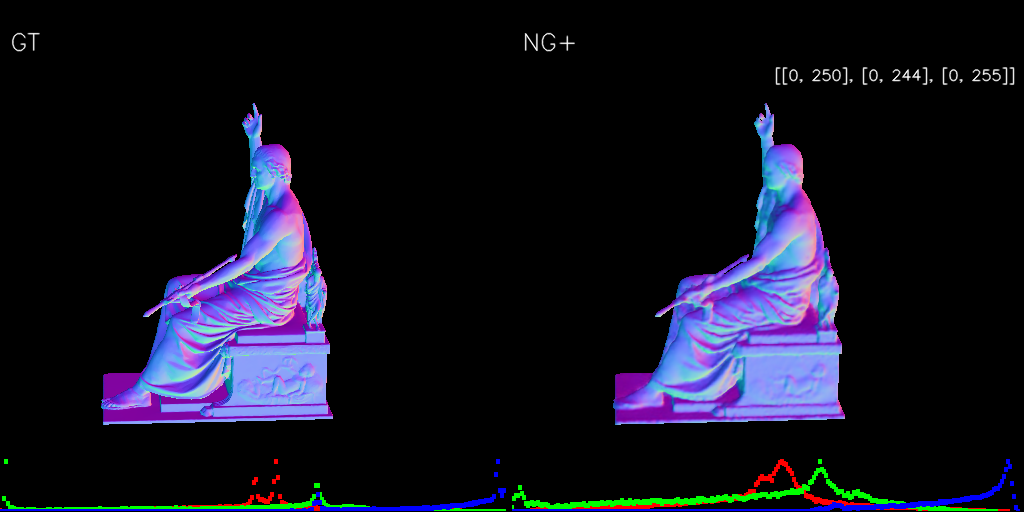
\includegraphics[width=\textwidth]{./pic/00349.gt.ngplus.png}}
%	\label{fig:washington_gt_ngpred}
%	\caption{Left: Ground truth normal map; Right: Predicted normal map based on model "NG"}
%\end{figure}

To further visualize the error of predicted normal map, figure \ref{fig:canny_edge_details} shows the angle error of normal map. 
It is obvious to see, that the error goes higher in the coarse surface, like fingers, gown and relief. Oppositely, the error goes lower in the smooth surface, like the arm, face, and foot. The coarse surface are mainly the boundaries, or edges, which can be extract efficiently using edge detection algorithms, like Canny Edge detector. Figure \ref{fig:canny_edge_details} shows the detected edge of ground truth using Canny Edge Detector.

%\begin{figure}[!h]
%	\centering
%	{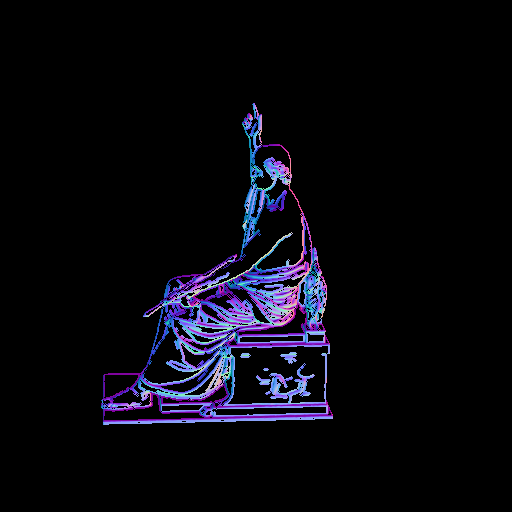
\includegraphics[width=0.45\textwidth]{./pic/00349.hpf0.png}}
%	{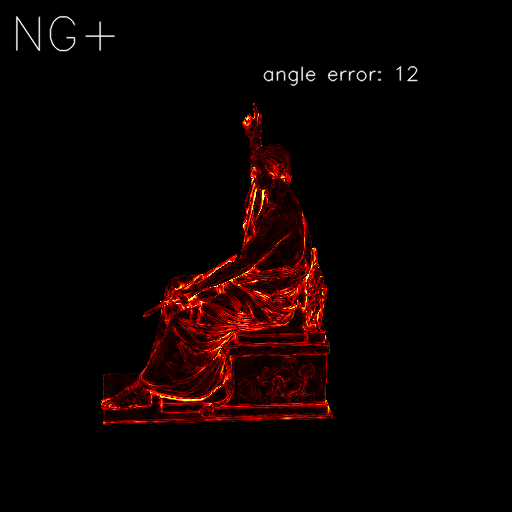
\includegraphics[width=0.45\textwidth]{./pic/00349.error.png}}
%	\label{fig:canny_edge_details}
%	\caption{Left: Normal Map; Middle: Detected Edge of Normal Map using Canny Edge Detection Algorithm; Right: Error of predicted normal map.}
%\end{figure}


\section{Detailed Gated ResNet Normal Neural Network}
Use edge detector algorithms for further improvement.



\newpage
\chapter{Formular}
RGB image will be stored as gray value Scene using following equation:
\[ gray: \frac{r+2g+b}{4}  \]



Capture Depth:
\[   \]


\subsection{Normal from k neighbors}

Given a point $ p $ locating on plane $ \Pi $, calculate the normal $ n $ of plane $ \Pi $. 

First, find the nearest $ k $ neighbors $ p_1,p_2,...,p_k $ of point $ p $ using KNN-algorithms. The plane $ \Pi $ containing point $ p $ can be fitted using the neighbors of point $ p $. Then the normal is available immediately.

Assume all the neighbors of point $ p $ are in plane $ \Pi = ax+by+cz+d=0 $. Since we only need calculate the normal, thus with out loss of generation, we can set displacement $ d = 0 $. Then the normal $  \bn = (a,b,c)^T  $.

Since all the neighbors of point $ p $ are located on plane $ \Pi $, thus we have 
\[ 
P_{k \times 3} \cdot  \bn_{3 \times 1} = \left(
\begin{matrix}
0 \\
0\\
0
\end{matrix}  \right) \]
In order to avoid trivial solution, one more constraint should be added
\[ \|  \bn_{3 \times 1} \|_2^2 = 1  \], which also let the normal to be a unit vector.
In order to calculate a valid normal, 3 points are required at least. For the sake of robust, more points can be used to reduce the measuring error. In this case, the equation system is over-determined, which can be modeled as following optimization problem
\begin{equation}
	\begin{array}{rrclcl}
		\displaystyle \min & \multicolumn{3}{l}{\| P  \bn \|^2} \\
		\\
		\textrm{s.t.} & \| \bn \|^2 & = & 1 
	\end{array}
\end{equation}
Let the decomposition of $ P=U\Sigma V^T $, The solution i.e. normal is the last column of $ V $.





\medskip

\bibliographystyle{plain}
\bibliography{reference}

\end{document}          
